\documentclass[journal]{IEEEtran}
\usepackage{graphicx}
\usepackage{subfigure}
\usepackage{cite}
\usepackage[justification=centering]{caption}
\graphicspath{{./figures/}}
\usepackage{makecell}
\usepackage{amsmath,amsfonts, amsthm}
\usepackage[ruled, linesnumbered]{algorithm2e}
\usepackage{algorithmic}
\newtheorem{definition}{Definition}
\newtheorem{theorem}{Theorem}
\newtheorem{lemma}{Lemma}
\usepackage{xcolor}
\usepackage{multicol}
\usepackage{multirow}
\usepackage{booktabs}
\usepackage{gensymb}
\usepackage{siunitx}
%\hyphenation{op-tical net-works semi-conduc-tor}
%\hyphenpenalty=6000
%\tolerance=10000
%\hbadness=10000

 \newcommand{\yjcomment}[1]{\textcolor{red}{#1}}


\begin{document}

\title{Customizable Data Trading via Blockchain: A Verifiable Approach Based on zk-SNARKs}

\IEEEtitleabstractindextext{%
    \begin{abstract}
       Data markets enable trading of datasets as commodities, responding to growing demand for analytics-ready information. However, exchanging raw data creates inherent privacy risks. Current solutions rely on one-size-fits-all anonymization – masking all datasets uniformly before release. This rigid approach becomes problematic because diverse analytical use cases require custom utility-privacy tradeoffs. To enable adaptive privacy, we propose a verifiable data trading framework using zk-SNARKs, smart contracts, and off-chain channels. Requesters specify custom masking rules while cryptographically verifying compliance via zero-knowledge proofs. We also propose a multi-round delivery scheme, enabling iterative quality validation with payment through off-chain channels. For dispute resolution, smart contracts verify zk-SNARK proofs of constraint adherence. Theoretical analyses demonstrate privacy preservation and verifiable integrity. The observed gas costs demonstrate the economic feasibility of our scheme for practical deployment.
    \end{abstract}
    \begin{IEEEkeywords}
        Blockchain, data trading, zero knowledge proof, zk-SNARK
    \end{IEEEkeywords} }

\maketitle
\IEEEdisplaynontitleabstractindextext
\IEEEpeerreviewmaketitle
 
\section{Introduction}
The exponential growth of cloud computing, blockchain, large language models, 5G communication, and Internet of Things (IoT) systems generates unprecedented volumes of high-value data. Within this ecosystem, data trading emerges as a core mechanism for maximizing data utility and enabling efficient value circulation in the data market\cite{marjanov2024sok}. 
As  data flow into trading markets—where owners monetize assets and requesters seek analytical value \cite{chen2014big}, a fundamental operational reality emerges: Data cannot change hands without inherent privacy exposure. Transfer, processing, or analysis inherently risks leakage, re-identification, or misuse. Thus, privacy preservation mechanisms become embedded in the transaction architecture.

This foundational need for privacy protection, however, creates a critical tension: Existing schemes predominantly rely on uniform masking/anonymization strategies\cite{zhang2024privacyasst}, yet this rigidity fails to accommodate diverse analytical requirements. Requesters exhibit heterogeneous needs—some prioritize fine-grained data, while others require only partial dimensions with basic anonymization. Consequently, one-size-fits-all approaches inevitably degrade data's intrinsic economic value.

To resolve this rigidity, we propose a paradigm shift toward flexible data trading: A framework enabling requester-specified privacy-utility tradeoffs. In this model, data owners possess sensitivity-containing datasets, while requesters not only select required plaintext fields but also define custom constraints and masking rules for sensitive attributes.  However, this customization introduces fundamental verification gaps regarding data compliance, and quality verification. Consider a \textit{Personal Health Record} (PHR) with fields $\mathcal{F} = \{\texttt{ssn}, \texttt{diagnosis}, \texttt{zip}, \texttt{age}\}$. A requester imposes distinct constraints per field: For $\texttt{ssn}$, $\mathcal{C}_1$ requires $\texttt{ssn}[0{:}2] = \texttt{"078"}$ (denoting New York issuance), with masking rule $\mathcal{M}_1(\texttt{ssn}) = \texttt{"***-**-}\chi_4\texttt{"}$ where $\chi_4 = \texttt{ssn}[7{:}]$ (exposing only the terminal four digits). For categorical $\texttt{diagnosis}$, $\mathcal{C}_2$ requires $\mathcal{M}_2(\texttt{diagnosis}) \in \{\texttt{cardiovascular}, \texttt{neurological}\}$. For $\texttt{zip}$, they require the plaintexts and  for $\texttt{age}$, suppression rules apply:  $\mathcal{M}_4(\texttt{age}) = \lfloor \texttt{age}/10 \rfloor \times 10$. The data compliance check includes verifying constraint compliance and data integrity. Data compliance verification without showing the original data is challenging, especially after data desensitization \cite{yamac2020multi, hong2023location}. A trivial solution is committing the data using a hash function and then applying zk-SNARKs using the entire record as input. However, this solution drastically escalates circuit complexity, incurring prohibitive overhead. Moreover, data quality remains unverifiable through compliance checks alone. Even with formally satisfied constraints, malicious owners can: (1) perturb SSNs to create semantically invalid but constraint-compliant values (e.g., $\texttt{ssn}' = \texttt{"078-00-0000"}$), and (2) adversarially select high-frequency diagnoses (e.g., consistently reporting $\texttt{cardiovascular}$) without violating syntactic rules. This violation is not detectable by zero-knowledge based payment schemes like ZKCP \cite{campanelli2017zero}. This dual challenge—prohibitive computational barriers for validity verification and undetectable generation of technically compliant but worthless data—fundamentally hinders the practical application of requester-specified privacy-utility tradeoffs.

In conventional data trading frameworks, trusted third-party intermediaries are frequently employed to perform critical functions including data compliance verification and quality assessment, such as DataWeb~\cite{dataweb}, Dawex~\cite{dawex}, and FactualData~\cite{factualdata}. However, centralized platforms present significant trust and reliability limitations. Both data owners and requesters must rely on these intermediaries to protect sensitive information~\cite{d2009user}, creating fundamental trust dependencies. Furthermore, their monolithic architectures introduce systemic vulnerabilities; notably, single points of failure may cascade into full trading ecosystem disruptions~\cite{dooley2001designing}.

To address these limitations, recent research has proposed blockchain-based decentralized data trading schemes~\cite{buterin2014next, an2021secure,chen2024two}. These systems leverage smart contracts to automate transaction execution and enhance transparency, thereby streamlining verification processes and fund management.  However, significant technical challenges persist when implementing such approaches in customizable data trading frameworks. The inherent public verifiability of smart contracts creates fundamental tension with essential privacy requirements.  Zk-SNARKs~\cite{ben2014succinct,groth2016size,gabizon2019Plonk} enable private data compliance verification through flexible circuit definition, yet their direct application faces efficiency challenges. Proof generation overhead scales with circuit complexity and input size, causing significant slowdowns when processing full compliant data check. For integrity verification, Merkle trees~\cite{islam2025multiple,song2023blockchain,aitzhan2016security} require data owners to commit roots to smart contracts, with Merkle proofs verifying leaf-to-root paths. However, plaintext proofs leak data scale through path depth~\cite{sun2020adaptive}. While using merkle proofs as private zk-SNARK inputs prevents plaintext exposure, the constraint count in resulting SNARKs may still reveal Merkle tree depth. Consequently, designing an efficient mechanism for simultaneous constraint verification and integrity proof with ensured privacy protection is a technical challenge. In addition, customizable data trading complicates quality assessment since masking hinders mutual ciphertext evaluation. Data assessment post-delivery is efficient but creates trust issues: requesters risk paying for low-quality data, while owners risk non-payment.  Designing a fair delivery protocol is crucial. 

In this paper, we propose a verifiable and customizable data trading scheme where data requesters verify custom constraints and integrity of masked data, while data owners preserve privacy and receive fair payments. Our solution employs a four-layer Merkle tree for efficient zk-SNARK proof construction, reducing blockchain storage and concealing data scale. For fair trading and data quality guarantee, we design a multi-round off-chain protocol to exchange data subsets against payment commitments. In addition, we introduce an on-chain dispute mechanism using zk-SNARKs to penalize malicious behavior. This mechanism limits the financial risk of low-quality data to a single subset. The contributions  are summarized as follows.
\begin{itemize}
    \item We propose a zk-SNARK and Merkle Tree based scheme for verifying customized data constraints and integrity without exposing sensitive information. Through the design of four-layer Merkle tree, the data compliance verification is highly efficient. 
    \item We design a multi-round off-chain delivery scheme with zk-SNARK-based dispute resolution, enabling  data quality assessment and fair payments. This mechanism confines the risk of paying for low-quality data to just one subset.
    \item We conduct comprehensive security and performance analyses to confirm the privacy preservation, verifiability, fairness of our scheme. The experiment results demonstrate the efficient zk-SNARK proof generation, and gas-efficient blockchain operation.
\end{itemize}  

The rest of this paper is organized as follows.
In Section \ref{section:related_work}, we present the related works about data trading, data desensitization, and data quality verification.
In Section \ref{section:preleminaries}, we introduce the preliminaries of zk-SNARK, blockchain, and off-chain channels.
In Section \ref{section:system_model}, we introduce the system model, threat model and security assumptions, and design goals.
The description of our proposed architecture is given in Section \ref{section:solution}.
We analyze the security of the proposed architecture in Section \ref{section:security_analysis}.
In Section \ref{section:performance_analysis}, we show the evaluation results of a series of experiments, and finally, we conclude and discuss the future work in Section \ref{section:conclusion}.

  
\section{Related Work} \label{section:related_work}
Sensitive information in collected datasets is commonly protected through desensitization techniques such as encryption \cite{yamac2020multi,eshun2024cryptographic}, data obfuscation \cite{hong2023location,li2023privacy}, k-anonymization \cite{hoang2023protecting}, and differential privacy \cite{hu2023federated}.   In data exchange scenarios (e.g., trading or sharing), data owners typically mask sensitive information (e.g., transforming geographic coordinates like \ang{39;54;22.6}N to \ang{39;54;}xxN) to preserve privacy prior to dissemination. However, a uniform masking strategy hinders optimal data utilization in case of varying requester requirements. Consequently, there is a critical need for data trading solutions that simultaneously ensure privacy protection and enable requesters to customize data constraints and to verify their fulfillment.

While effective for ensuring confidentiality, the aforementioned methods universally lack robust verification mechanisms. This deficiency manifests in two critical limitations: (1) data requesters cannot verify that original data actually satisfies their specific constraints, and (2) requesters cannot confirm the integrity of the received data, making it difficult to determine whether the data was genuinely processed from the original source or artificially fabricated. The emergence of blockchain technology \cite{buterin2013ethereum} and advances in zero-knowledge proofs (ZKPs) \cite{ben2014succinct,groth2016size,gabizon2019Plonk} have enabled approaches that utilize smart contracts for public logic verification while employing ZKPs to validate data constraints. Protocols such as Zero-Knowledge Contingent Payment (ZKCP) \cite{campanelli2017zero} and Fairswap \cite{dziembowski2018fairswap} require data owners to submit ZKPs demonstrating fulfillment of data requests. However, these approaches exhibit significant limitations: ZKP generation remains computationally intensive. More critically, they lack robust mechanisms for data quality assessment when handling complex, flexible data masking requirements.  This deficiency enables potential exploitation: a malicious data owner could leverage a minimal valid dataset, iteratively applying minor modifications to generate large volumes of effectively homogeneous data that satisfy zero-knowledge proof constraints while offering limited utility.  Consequently, prior works fail to meet our scenario's stringent requirements for comprehensive data quality verification. Furthermore, the diversity of data masking requirements in our scheme impedes the establishment of a unified quality evaluation framework \cite{zhao2019data,zhao2020pace}. 

To ensure transaction fairness while enabling data requesters to evaluate data quality, an efficient approach leverages multiple granular transactions through off-chain channels \cite{luo2024crosschannel}. This mechanism requires the data owner to strategically partition the target dataset into discrete subsets, exchanging each fragment incrementally for corresponding payment commitments via secure off-chain channels. Crucially, this framework empowers data requesters to terminate transactions upon detecting substandard quality in any subset, thereby limiting financial risk. Simultaneously, the system protects data owners. It ensures requesters cannot access significant data volumes without payment. Despite its operational simplicity and efficiency, this approach exhibits significant vulnerabilities. Malicious requesters may repudiate payment obligations after receiving sequential data transfers, while dishonest data owners might withhold committed data segments after securing partial payments. These adversarial exploitation vectors necessitate the design of a more robust data delivery mechanism with enhanced fairness guarantees.


\section{Preliminaries}\label{section:preleminaries}

\subsection{Zero Knowledge Succinct Non-interactive Argument of Knowledge (zk-SNARK)}\label{subsec:zk-SNARK}

Zk-SNARK \cite{ben2014succinct} is a succinct non-interactive zero-knowledge proof system comprising three polynomial-time algorithms: 
$\text{Setup}$, $\text{Prove}$, and $\text{Verify}$. It satisfies perfect completeness, succinctness, computational zero-knowledge, and simulation extractability.


\begin{itemize}
    \item $\mathsf{Setup}(1^\lambda, \mathcal{C})$: This algorithm takes a security parameter $\lambda$ and a circuit $\mathcal{C}$ as input, and outputs a common reference string $crs$ which contains the proving key $\mathbf{pk}$ and the verification key $\mathbf{vk}$.
    \item $\pi \leftarrow \mathsf{Prove}(crs, \mathcal{R}, x, w)$: This algorithm takes the common reference string $crs$, a public statement $x$, and a private witness $w$ as input, and generates a proof $\pi$. 
    \item $b \leftarrow \mathsf{Verify}(crs, \mathcal{R}, x, \pi)$: This algorithm takes the common reference string $crs$, a statement $x$, and a proof $\pi$ as input, and outputs a boolean value. The output is \textit{true} for a valid proof and \textit{false} otherwise.
\end{itemize}

Zk-SNARKs have gained significant attention in privacy-preserving applications and blockchain systems due to their ability to generate succinct proofs and enable efficient verification \cite{sasson2014zerocash}. They allow complex computations to be verified without revealing input information, making them essential for use cases requiring both strong privacy and verifiable correctness \cite{kosba2016hawk}.



\subsection{Blockchain and Smart Contract}
Blockchain technology, popularized by Bitcoin's implementation \cite{nakamoto2008bitcoin}, operates as a distributed ledger maintaining immutable and transparent transaction records. Ethereum \cite{buterin2013ethereum} extends this foundation through smart contracts—self-executing programs enabling complex computational logic and automated agreement enforcement without intermediaries. A critical feature of smart contracts is their public verifiability, particularly valuable for data trading ecosystems. First, they can validate plaintext data constraints to ensure traded information meets specifications. Second, and more importantly for privacy, they enable on-chain verification of zk-SNARK proofs without accessing underlying private data. This creates a trustless verification mechanism where computation correctness over private inputs is publicly verifiable while preserving confidentiality \cite{wan2022zk}. In our scheme, we leverage these capabilities to implement a verification contract as the core dispute resolution mechanism in data delivery processes.


\subsection{Off-chain Channel}\label{subsec:off_chain_channel}
Off-chain channels were initially conceived as payment channels \cite{poon2016bitcoin} to improve blockchain scalability. In this approach, two parties lock funds on-chain as collateral, conduct numerous transactions off-chain, and only submit the final settlement to the blockchain. This significantly reduces on-chain transactions and associated costs. The concept later evolved into state channels \cite{dziembowski2018general}, which generalize beyond simple payments to handle arbitrary state transitions. Parties interacting within a state channel can update state off-chain while retaining the ability to resolve disputes on-chain. By keeping intermediate states off-chain and recording only the final state on the blockchain, this mechanism not only improves transaction throughput but also enhances privacy through confidential state transitions \cite{qin2023blindhub}.


\section{System model, Motivation, Security assumptions and Design Goals}\label{section:system_model}

\subsection{System Model}

\begin{figure}[htbp]
    \centering
    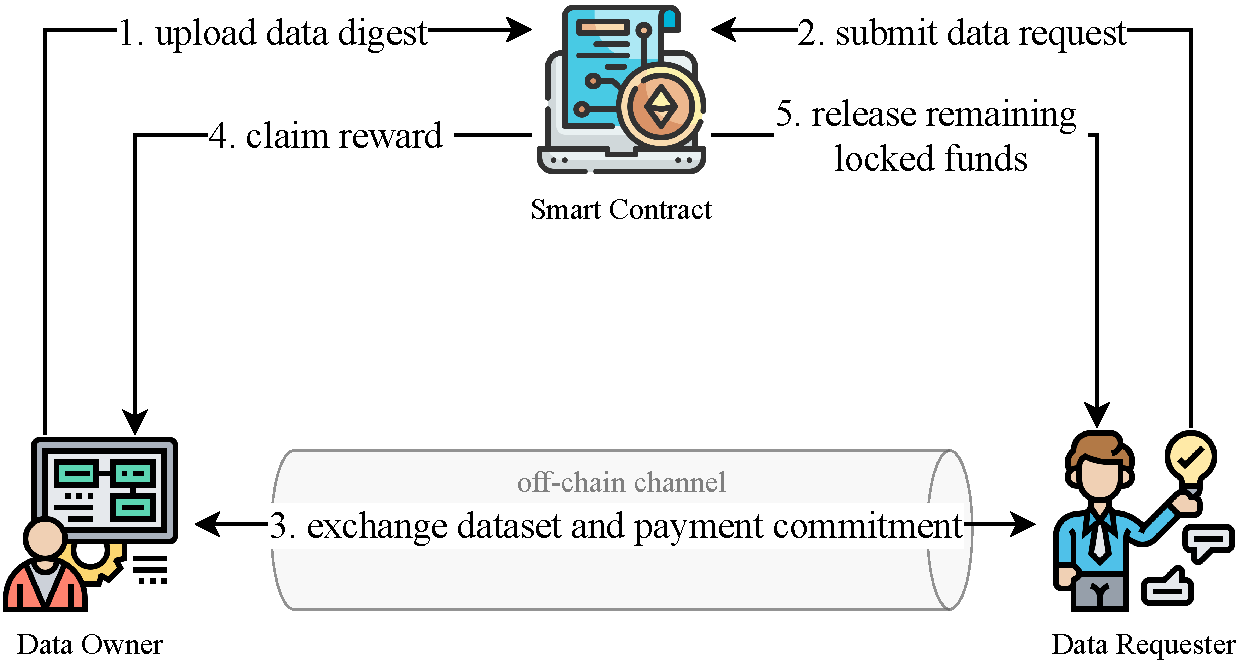
\includegraphics[width=1.0\linewidth]{figures/scheme/system-model.pdf}
    \caption{Scheme Overview}\label{fig:system-model}
\end{figure}

As depicted in Fig.~\ref{fig:system-model}, the system has the following roles and they function as follows.

\subsubsection{\textbf{Data Owner} ($\mathcal{DO}$)}

Data owner $\mathcal{DO}$ collects valuable data through their devices and systems. Upon receiving a data request that includes constraints for sensitive information and masking rules, $\mathcal{DO}$ filters out datasets that meet the constraints and apply the masking rules to the requested sensitive information to generate \textit{tailored datasets}. $\mathcal{DO}$ and data requester $\mathcal{DR}$ complete the data delivery through an off-chain channel, the datasets are only provided upon receiving a valid payment commitment from $\mathcal{DR}$.

\subsubsection{\textbf{Data Requester} ($\mathcal{DR}$)}

Data requesters $\mathcal{DR}$ submit a data request to $\mathcal{DO}$ with sensitive information constraints and corresponding masking rules. $\mathcal{DR}$ and $\mathcal{DO}$ interact multiple rounds through an off-chain channel to deliver datasets. $\mathcal{DR}$ only provides the payment commitment for the current round if the tailored dataset and the corresponding proof are verified as valid. If satisfied with the data quality, $\mathcal{DR}$ then provide the validity proof for the payment commitment of the next round. 

\subsubsection{\textbf{Smart Contracts}}

To minimize on-chain computational overhead, the data trading process is primarily conducted off-chain, with only financial transactions and dispute resolution mechanisms implemented on-chain. Our system employs two distinct smart contracts: 
(1) the Data Contract ($\mathsf{DC}$), deployed by Data Owners ($\mathcal{DO}$s), stores data digests and associated metadata; 
and (2) the Verification Contract ($\mathsf{VC}$), deployed by Data Requesters ($\mathcal{DR}$s), manages transaction funds and $\mathcal{DO}$ deposits while incorporating zk-SNARK proof verification to resolve data delivery disputes.

\subsection{Threat Model and Security Assumptions}\label{subsec:threat_model}
Following related data trading schemes~\cite{campanelli2017zero}, we model both Data Owners ($\mathcal{DO}$) and Data Requesters ($\mathcal{DR}$) as potentially malicious. A malicious $\mathcal{DO}$ may seek illegitimate reward by providing fabricated, tampered, or low-quality data. A malicious $\mathcal{DR}$ may attempt to compromise privacy by inferring sensitive information—such as specific data content or scale—from the proofs supplied by the $\mathcal{DO}$, or may try to acquire data without providing the required payment.

Regarding the underlying infrastructure, we assume the blockchain is secure and tamper-proof. We further assume that the off-chain channel between a $\mathcal{DO}$ and a $\mathcal{DR}$ is secure and resistant to eavesdropping by unauthorized third parties.

\subsection{Design Goals}\label{subsec:design_goals}
We aim to design a customizable and verifiable data trading scheme which allows the $\mathcal{DR}$ to verify the validation of constraints and integrity of tailored datasets, and to evaluate their quality without leaking sensitive information from the original dataset. To achieve this goal, we propose the following detailed design goals.

\subsubsection{\textbf{Data Privacy Preservation}}
The proposed scheme should enable the $\mathcal{DO}$ to trade data while ensuring privacy preservation. $\mathcal{DO}$ can prove to $\mathcal{DR}$ that the masked data in the tailored dataset is processed from the original dataset without exposing sensitive information like data content or data scale.

\subsubsection{\textbf{Verifiability of Masked Data Constraint and Integrity}} 
$\mathcal{DR}$s should possess the capability to verify both the constraint validity and integrity of received data. Specifically, even when data is processed through masking rules, $\mathcal{DR}$s should be able to validate whether the received data satisfy their custom constraints. Furthermore, $\mathcal{DR}$s need to verify that the received masked data is indeed derived from endorsed original data through specified masking rules, and that no tampering has occurred during the processing procedure.

\subsubsection{\textbf{Data Delivery Fairness}}
The scheme enforces fairness in data trading by preventing: (i)~$\mathcal{DO}$ payment without valid data delivery, and (ii)~$\mathcal{DR}$ data access without payment. Dispute resolution addresses malicious behavior. Given smart contracts' inability to assess data quality, we introduce \emph{acceptable fairness}: by partitioning data into low-value subsets (where $\textit{value}_{subset} \ll \textit{value}_{dataset}$), $\mathcal{DR}$'s maximum loss is bounded to one subset's cost, making quality-related financial risk negligible while preserving core exchange guarantees.

\section{Our Proposed Solution}\label{section:solution}

\subsection{Overview}

\begin{figure}[htbp]
    \centering
    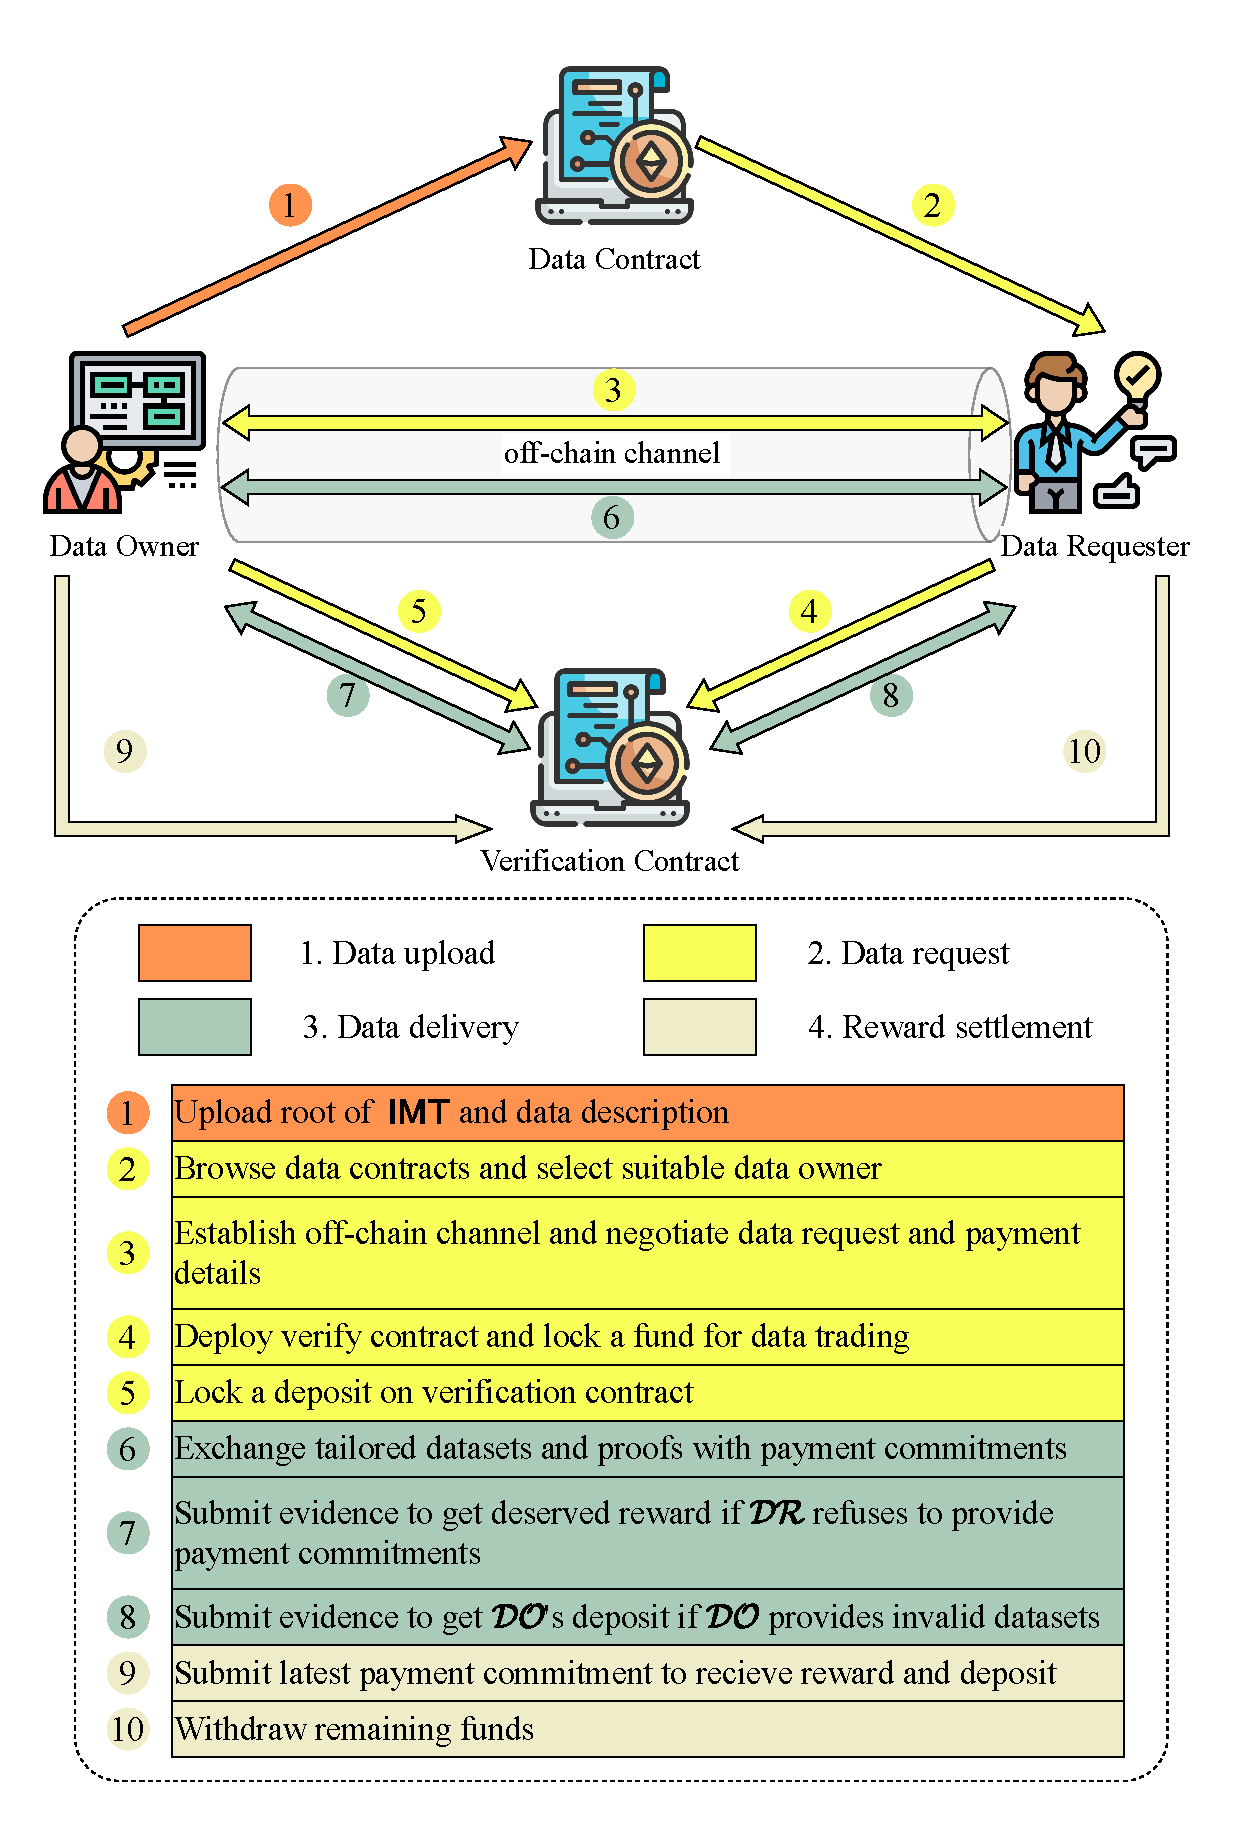
\includegraphics[width=1.0\linewidth]{figures/scheme/detailed-process.pdf}
    \caption{Detailed Process in Our  Scheme}\label{fig_detail_process}
\end{figure}
We propose a customizable and verifiable data trading scheme, consisting of data integrity and constraints proof scheme and multi-round fair data exchange process. To efficiently prove the integrity and customizable constraints of masked data without leaking any sensitive information and reduce the storage burden on blockchain, we propose a data integrity and constraints proof scheme based on zk-SNARK and a four-layer Merkle Tree, denoted as Integrity Merkle Tree ($\mathsf{IMT}$). To enable data requester to assess data quality while ensuring data owner receive due payment, we introduce off-chain channel and multi-round data delivery process. During multi-round data delivery, the data owner may maliciously refuse to pay for the received subset. To address this potential malicious behaviors, we design a dispute resolution mechanism based on zk-SNARK proof verification on smart contract. The work flow of our scheme can be summarized as follows:
\begin{enumerate}
    \item \textbf{Data upload.} 
    $\mathcal{DO}$ organizes the collected datasets into $\mathsf{IMT}$ and submit the root of $\mathsf{IMT}$ and corresponding data description on his/her data contract, denoted as $\mathsf{DC}$, which corresponds to step 1 in Fig.~\ref{fig_detail_process}.
    
    \item \textbf{Data request.} 
    $\mathcal{DR}$ and $\mathcal{DO}$ establish an off-chain channel to negotiate specific data requests and payment details. Once $\mathcal{DO}$ and $\mathcal{DR}$ reach a consensus, $\mathcal{DR}$ deploys a verification contract based on his/her data request, locks a fund in verification contract and uploads the anchor of a hash chain $H^{(n)}$ as a verifiable payment commitment. Subsequently, $\mathcal{DO}$ also locks a fund in verification contract as a security deposit to ensure that the data provided later is valid and untampered. The entire process corresponds to step 2, 3, 4, 5 in Fig.~\ref{fig_detail_process}.
    
    \item \textbf{Data delivery.}
    $\mathcal{DO}$ processes datasets into tailored datasets and divide the datasets into multiple subsets. For each tailored data subset, $\mathcal{DO}$ generates zk-SNARK proofs. $\mathcal{DO}$ exchanges data subsets with $\mathcal{DR}$ for payment commitments. The exchange round continues until the locked funds of $\mathcal{DR}$ are exhausted or a dispute arises. The entire process corresponds to step 6, 7, 8 in Fig.~\ref{fig_detail_process}.
    
    \item \textbf{Reward settlement.}
    $\mathcal{DO}$ can claim corresponding reward from the verification contract using the latest payment commitment, thereby completing the multi-round data delivery process. If the proof is invalid, $\mathcal{DR}$ can submit the data and proof on verification contract. If the proofs are invalid , $\mathcal{DR}$ can obtain the deposit from $\mathcal{DO}$ as a penalty for forging the proof.  The entire process corresponds to step 9, 10 in Fig.~\ref{fig_detail_process}.
    
\end{enumerate}

\subsection{Definition of Data Model and Merkle Tree}

\begin{figure}[htbp]
    \centering
    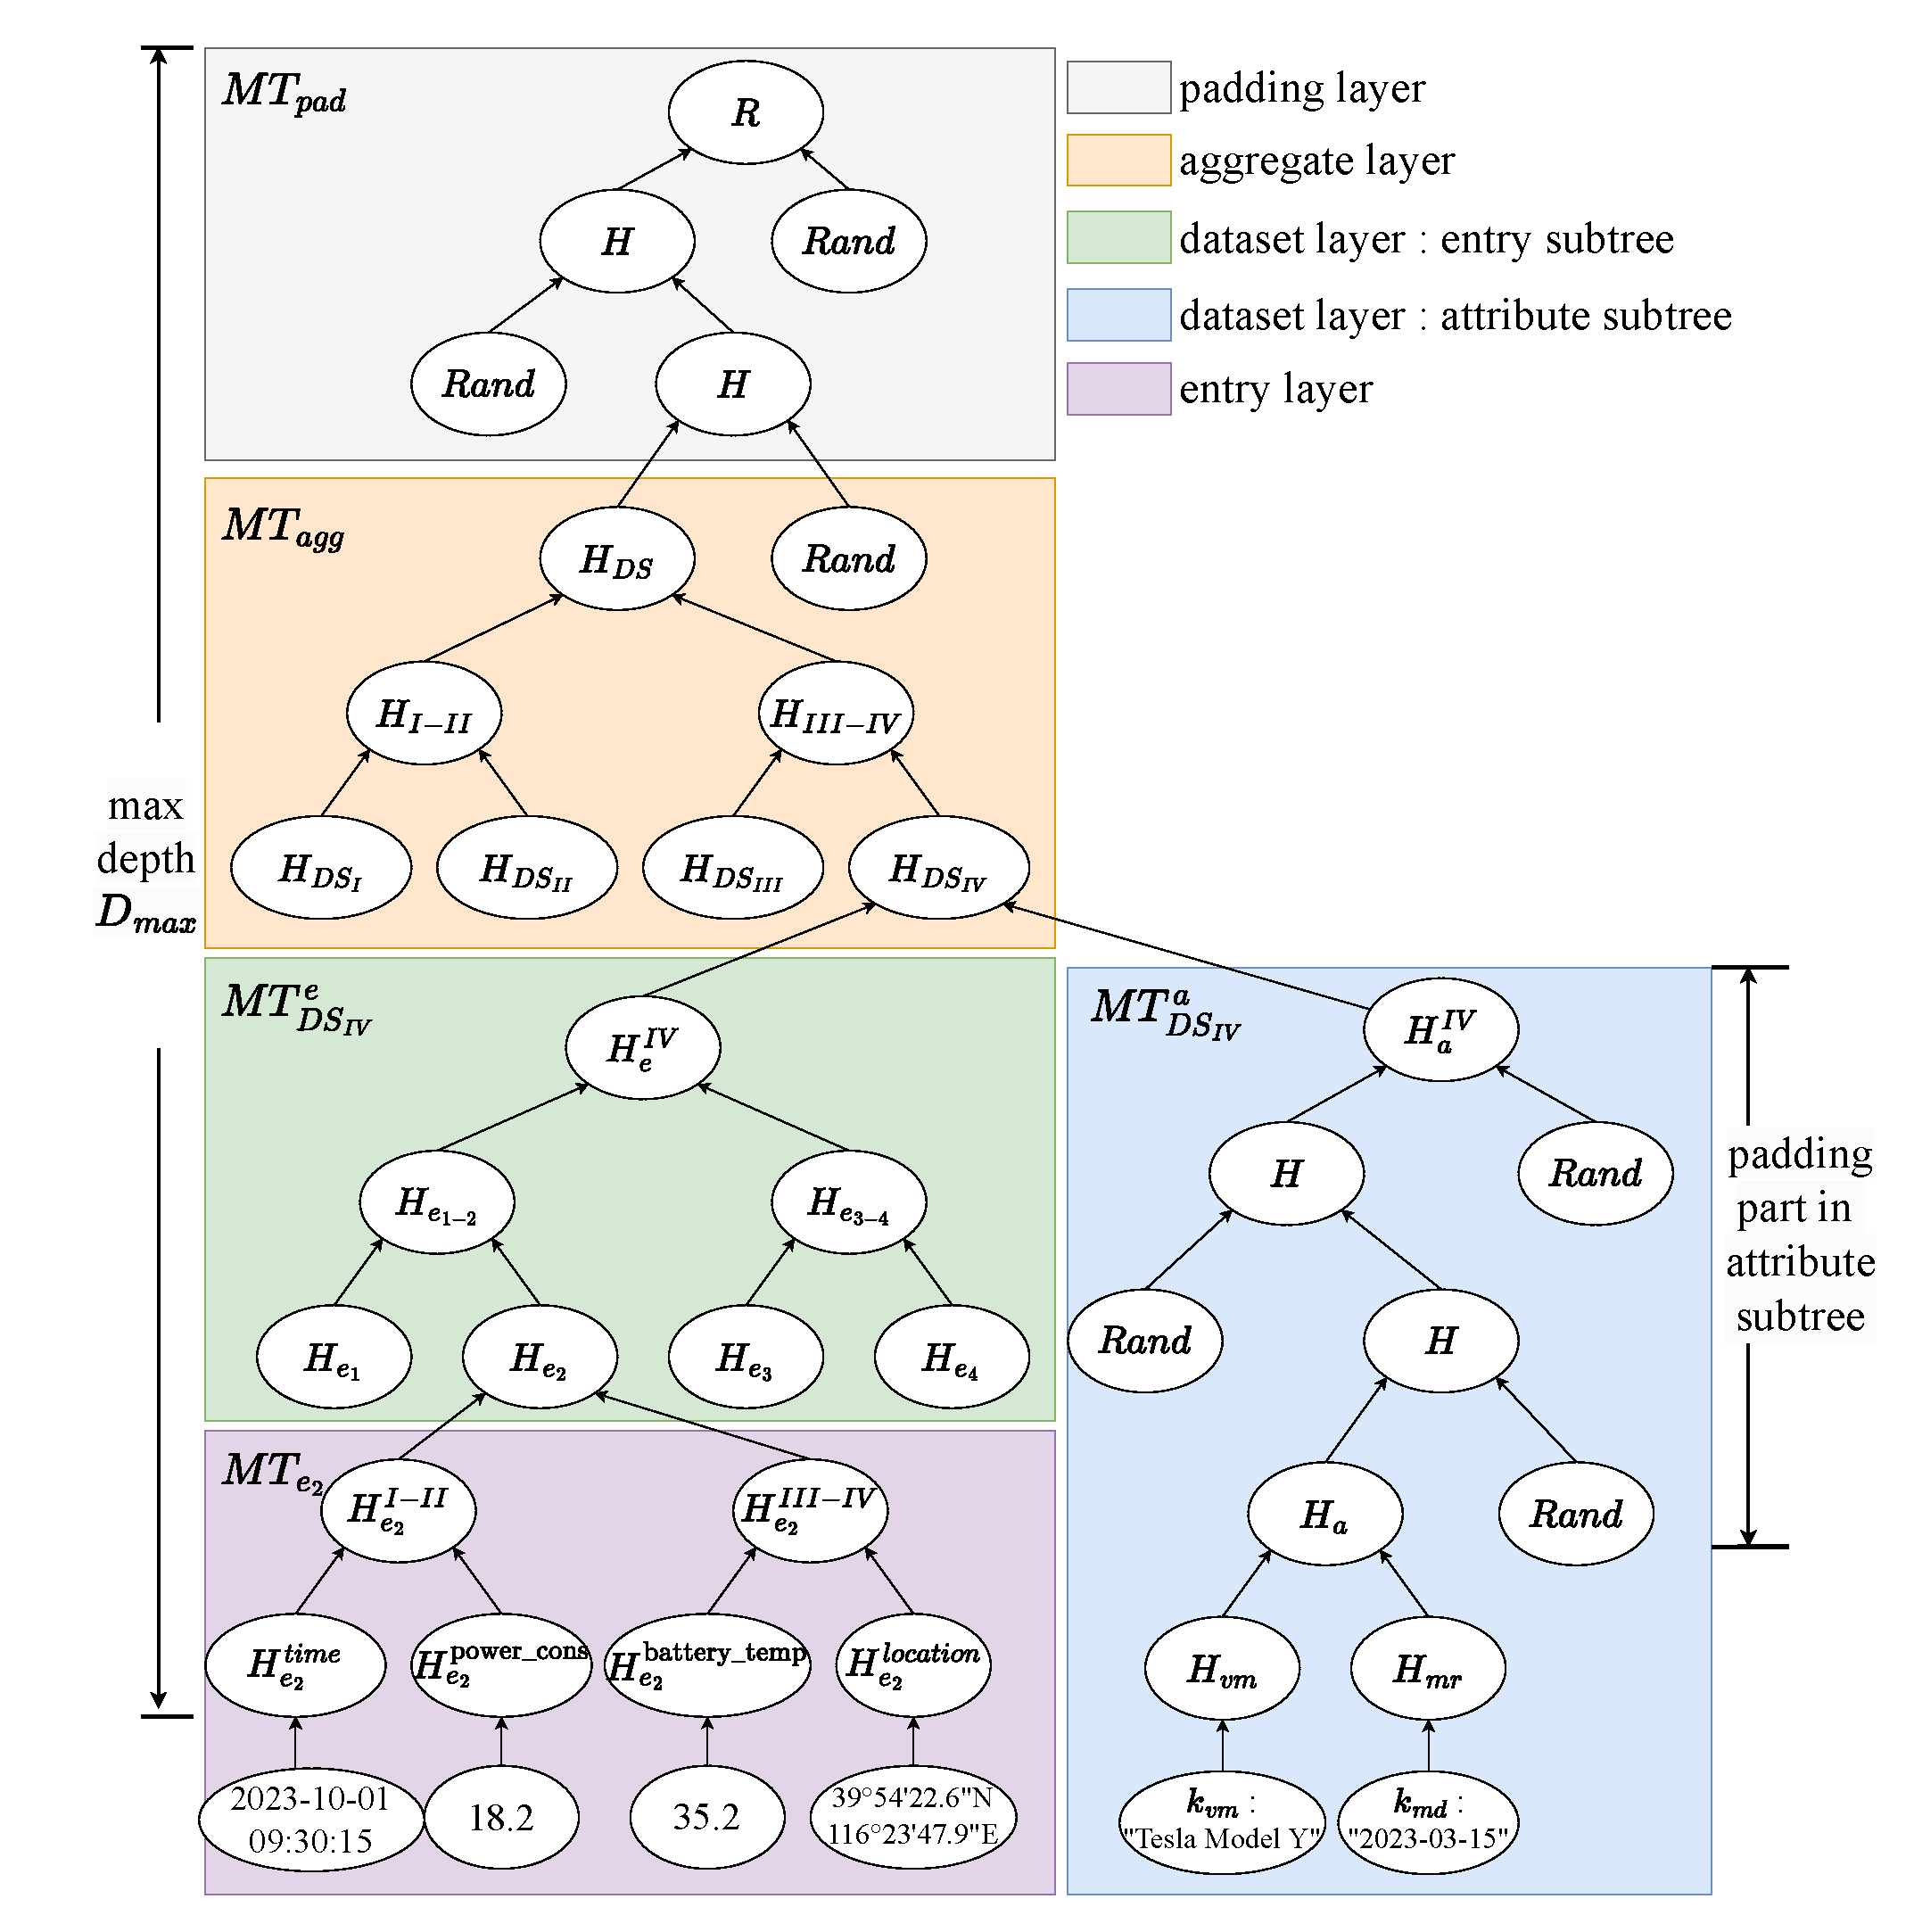
\includegraphics[width=1.0\linewidth]{figures/scheme/IMT.pdf}
    \caption{Example of $\mathsf{IMT}$}\label{fig:IMT}
\end{figure}

In blockchain-based data trading systems, efficiently representing complex datasets while maintaining verifiability presents significant challenges. Traditional Merkle tree implementations often struggle with: 1) supporting fine-grained data access at the field level, 2) accommodating heterogeneous data types within a unified structure, and 3) enabling efficient zero-knowledge proofs for selective disclosure. To address these challenges, we propose a hierarchical four-layer Merkle tree structure called Integrity Merkle Tree $\mathsf{IMT}$ that separates static attributes from dynamic entries while supporting field-level granularity. This design enables efficient generation of zk-SNARK proofs for selective data disclosure, reduces computational overhead by minimizing hash input lengths, and maintains consistent proof structures through strategic padding. Our approach allows $\mathcal{DO}$ to publish only a single root hash while supporting complex data queries and constraint verification. To facilitate the construction of the Merkle Tree and zk-SNARK proof, we present the detailed definition of data model in our scenario. 

\textbf{1) Definition of Data Model}. 

We define a dataset as the collection of all relevant data about an entity or an event gathered by a data owner. For example, all clinical records of a patient within a hospital, or all driving and perception data collected from an electric vehicle over a period of time.
We categorize the data type of dataset into two types: attribute information and entry information.  A dataset $DS$ is defined as a two-tuple $DS = \{A, E\}$, where $A$ represents the attribute set and $E$ represents the entry set. These two components are mutually exclusive and together constitute a complete dataset that can represent time-series data or event-based information collected from specific scenarios. The attribute set $A$ consists of a collection of key-value pairs that describe the static characteristics of the dataset, formally defined as $A = \{(k_i, v_i) | k_i \in K, 1 \leq i \leq p\}$, where $K$ is the attribute key set, $p$ is the number of key-value pairs, $k_i$ is the attribute key, and $v_i$ is the corresponding attribute value. The entry set $E$ comprises a collection of data records with identical structure that store the dynamic values of the dataset, formally defined as $E = \{e_i | e_i = (e_i^{f_1}, e_i^{f_2}, ..., e_i^{f_t}), f_j \in F, 1 \leq i \leq q, 1 \leq j \leq t\}$, where $F = \{f_1, f_2, ..., f_t\}$ is the field set, $q$ is the number of entries, $t$ is the dimension of each entry, $e_i^{f_j}$ represents the value of the $i$-th entry in field $f_j$, and $e^{f_j}$ denotes the sequence of values in field $f_j$ across all entries.

\textbf{2) Definition of $\mathsf{IMT}$}.

We design a four-layer Merkle tree as Integrity Merkle Tree $\mathsf{IMT}$, on one hand, to efficiently construct validity proofs for data constraints and integrity proofs using zk-SNARK, on the other hand, to reduce the blockchain storage burden by avoid uploading all datasets from data owner directly to the smart contract. Throughout the construction, we use a collision-resistant hash function $\mathcal{H}: \{0,1\}^* \rightarrow \{0,1\}^\lambda$ where $\lambda$ is the security parameter. From bottom to top, $\mathsf{IMT}$ consists of the Entry Layer, Dataset Layer, Aggregate Layer and Padding Layer.

\textbf{Entry Layer}. Each data entry $e_i$ forms a Merkle tree $MT_{e_i}$, where the leaf nodes ${H}_{e_i}^{f_j}$ correspond to the hash values of the entry's values combined with a random salt $r_{e_i}^{f_j}$ in each field $f_j$, where $H^{f_j}_{e_i} = \mathcal{H}(e_i^{f_j} || r_{e_i}^{f_j})$. This fine-grained design allows $\mathcal{DR}$ to specify requirements for each field individually while improving the efficiency of zk-SNARK proof generation by reducing the input length of hash proofs.

\textbf{Dataset Layer}. Each dataset $DS_i$ forms a Merkle tree $MT_{DS_i}$ containing two parts: attribute subtree $MT_{DS_i}^a$ and entry subtree $MT_{DS_i}^e$:
\begin{itemize}
    \item The leaf nodes of the attribute subtree are the hash values of key-value pairs with a random salt $r_{k_i}$, the resulting hash value is $\mathcal{H}(k_i || v_i || r_{k_i}), 1\leq i \leq p$.
    \item The leaf nodes of the entry subtree are the root nodes $H_{e_i}, 1\leq i \leq q$ from the Entry Layer.
\end{itemize}
The root $H_{DS_i}$ of the merged tree serves as the digest of dataset $DS_i$.

\textbf{Aggregate Layer}. The Merkle tree in aggregate layer is constructed using the digests of multiple datasets $H_{DS_1}, H_{DS_2}, ..., H_{DS_n}$ as leaf nodes, resulting in the root node $H_{DS}$. This aggregation is designed to reduce blockchain storage overhead by uploading a single aggregated root hash instead of individual dataset roots, making the system more scalable and cost-effective.

\textbf{Padding Layer}. To preserve the dataset scale information, $\mathcal{DO}$ pre-defines a maximum tree depth $D_{max}$ and extends the total tree depth to $D_{max}$ through random padding. By ensuring all $\mathsf{IMT}$ have identical depth $D_{max}$, the padding mechanism prevents information leakage about both the number of data entries within individual datasets and the number of datasets aggregated in each $\mathsf{IMT}$, thereby preserving data owner's privacy regarding their data scale. The padding does not require forming a complete binary tree. It only needs to ensure the existence of a Merkle path with depth $D_{max}$. Padding nodes can be randomly selected as left or right subtrees like in Fig.~\ref{fig:IMT}.

As shown in Fig.~\ref{fig:IMT}, we demonstrate the four-layer construction of $\mathsf{IMT}$ using a simplified electric vehicle dataset. In this example dataset, the entry information contains electric vehicle data that dynamically changes with time, including four fields: time, power consumption, battery temperature, and location. To facilitate fine-grained data requests targeting specific fields within the entry information, the leaf nodes in entry layer are designed as hash of entry $e_2$'s specific values across the four fields, corresponding to $H^{time}_{e_2}$, $H^{power\_cons}_{e_2}$, $H^{battery\_temp}_{e_2}$, and $H^{location}_{e_2}$. Four entries $e_1$, $e_2$, $e_3$, and $e_4$ form an entry subtree in dataset layer as $H^{IV}_e$. 
The attribute information contains the static characteristics in the electric vehicle dataset, which in this case includes the vehicle model and manufacture date. The leaf nodes of the attribute subtree in dataset layer are hash values of the vehicle model and manufacture date, corresponding to $H_{vm}$ and $H_{mr}$. It is important to note that, due to space constraints of Fig.~\ref{fig:IMT}, the random salts are not depicted, so that we can focus on illustrating the essential hierarchical structure of $\mathsf{IMT}$.
The attribute subtree requires padding to achieve equal depth from $H_{vm}$ to $H^{IV}_e$ and $H^{time}_{e_2}$ to $H^{IV}_e$. This design ensures a consistent and fixed number of constraints when subsequently generating zk-SNARK proofs based on Merkle proofs. The $H^{IV}_e$ and $H^{IV}_a$ of dataset $DS_{IV}$ jointly form the leaf node $H_{DS_{IV}}$ in the aggregate layer. 
At the aggregation layer, the hash values of four datasets, $H_{DS_{I}}$, $H_{DS_{II}}$, $H_{DS_{III}}$, and $H_{DS_{IV}}$ are combined to construct a Merkle tree $H_{DS}$. Due to potential variations in the quantity and scale of datasets collected across different batches, a padding layer is added above the aggregation layer to maintain consistent depths of $\mathsf{IMT}$. This design ensures that the overall depth of the $\mathsf{IMT}$ reaches the predetermined maximum value $D_{max}$, thereby guaranteeing uniform constraint numbers during subsequent generation of zk-SNARK proofs. After padding $\mathsf{IMT}$ to root $R$, $\mathcal{DO}$ uploads $R$ and corresponding data description on his/her data contract, denoted as $\mathsf{DC}$.

\subsection{Customizable Data Request and Verification Mechanism}

In data trading ecosystems, a fundamental challenge exists in balancing granular data access with privacy preservation. Traditional approaches either expose excessive information during verification or limit request flexibility. Data requesters need to specify complex constraints on both static attributes and dynamic entries while data owners must provide verifiable evidence of compliance without revealing sensitive information about their datasets. To address these challenges, we propose a  request-verification framework with two key components: (1) a structured data request model supporting both plaintext and masked data delivery, and (2) complementary zero-knowledge proof mechanisms that verify constraint satisfaction and data integrity while preserving privacy.

\textbf{1) Customizable Data Request}.

In our scheme, a data request $R$ consists of two parts, the attribute request and the entry request, formally defined as $R=\{R_a,R_e\}$. Each request further contains plaintext request and masking request components.

\textbf{Attribute Request}. The attribute request $R_a$ comprises plaintext attribute request $R_a^p$ and masking attribute request $R_a^m$, formally defined as $R_a = \{R_a^p,R_a^m\}$:

\begin{itemize}
    \item The plaintext attribute request $R_a^p$ is defined as $R_a^p=\{(k_i,c_i^a) | k_{i}\ \in K_{R_{a}^{p}}\}$, where $K_{R_{a}^{p}}$ is the plaintext attribute key set and $K_{R_{a}^{p}} \subseteq K$. $c_i^a$ represents the constraint condition for the attribute $k_i$. If $c_i^a =\emptyset$, the value $v_i$ of attribute $k_i$ is provided directly. If $c_{i}^a\neq \emptyset$, only values satisfying $v_{i}\models c_{i}^a$ are provided. For example, $R_a^p=\{(\text{vehicle model},\text{=Tesla Model Y}), (\text{battery capacity},\emptyset)\}$ requests the vehicle model must be Tesla Model Y and battery capacity without constraints.
    \item The masking attribute request $R_a^m$ is defined as $R_a^m=\{(k_{i},c_{i}^a,mr_{i})| k_{i}\ \in K_{R_{a}^{m}}\}$, where in addition to the attribute key $k_i$ and condition $c_i^a$, a masking rule $mr_i$ is specified. For example, $R_a^m=\{(\text{manufacture date}, year=2020, \texttt{YYYY-XX-XX})\}$ requests the manufacture date from 2020, masked in the format $\texttt{YYYY-XX-XX}$.
\end{itemize}


\textbf{Entry Request}. Similarly, the entry request $R_e$ consists of plaintext field request $R_e^p$ and masking field request $R_e^m$, formally defined as $R_e=\{R_e^p,R_e^m\}$:

\begin{itemize}
    \item The plaintext field request $R_e^p$ is defined as $R_e^p=\{({f_{i}},c_{i})|f_{i} \in F_{R_e^p}\}$, where $F_{R_{e}^{p}}$ is the plaintext field set and $F_{R_{e}^{p}} \subseteq F$. For example, $R_e^p=\{(\text{time},\text{year=2023}),(\text{power cons},\emptyset),(\text{battery temp},\emptyset)\}$ requests time entries from 2023, along with unconstrained power consumption and battery temperature values.
    \item The masking field request $R_e^m$ is defined as $R_e^m=\{(f_{i},c_{i}^f,mr_{i})| f_{i} \in F_{R_{e}^m}\}$, where $F_{R_{e}^{m}}$ is the masking field set and $F_{R_{e}^{m}} \subseteq F$. For example, $R_e^m=\{(\text{location}, \{lat \in [\ang{39;49;55.22}N, \ang{39;59;2.47}N] \land lon \in [\ang{116;16;40.39}E, \ang{116;28;54.94}E]\},\text{precision}=1')\}$ requests location data within specified latitude and longitude ranges, masked to minute precision.
\end{itemize}

\textbf{2) Verification Mechanism Based on zk-SNARKs}.

The granular request structure creates new verification challenges: how to prove that (1) the provided data satisfies the specified constraints, and (2) the data originates from the endorsed dataset, all without revealing sensitive information about the dataset structure or content. To solve these challenges, we design two complementary proof mechanisms: Constraint-Hash Proof and Root Obfuscation Proof.

\textbf{Constraint-Hash Proof}. The constraint-hash proof binds the validity verification of data content with hash values through zero-knowledge proof techniques. For attribute value $v_i$ and entry field value $e_j^{f_t}$, the proofs are generated in the following forms:

For attribute values, the definition of constraint-hash proof can be denoted as:
\begin{equation}
\begin{aligned}
     \pi_{a}^{CH}(k_i, v_i) = \mathsf{ZKP} & \bigg\{ (k_i, v_i, r_{k_i}; h_i) : \\ 
    & v_i \models c_i^a \land \mathcal{H}(k_i || v_i || r_{k_i}) = h_i \bigg\},
\end{aligned}
\label{eq:proof_cha}
\end{equation}
where $k_i, v_i$ and random salt $r_{k_i}$ is the private input and the $h_i$ is the public input of zk-SNARK proof $\pi_{a}^{CH}(v_i)$.

For entry field values, the definition of constraint-hash proof can be denoted as:
\begin{equation}
\begin{aligned}
        \pi_{e}^{CH}(e_j^{f_t}) = \mathsf{ZKP} & \bigg\{(e_j^{f_t}, r_{e_j}^{f_t}; h_j^{f_t}) : \\ 
        & e_j^{f_t} \models c_t^f \land \mathcal{H}(e_j^{f_t} || r_{e_j}^{f_t}) = h_j^{f_t}\bigg\},
\end{aligned}
\label{eq:proof_che}
\end{equation}
where $e_j^{f_t}$ and random salt $r_{e_j}^{f_t}$ is the private input and the $h_j^{f_t}$ is the public input of zk-SNARK proof $\pi_{e}^{CH}(e_j^{f_t})$.

This constraint-hash binding design ensures that the proven hash values indeed correspond to data satisfying the constraints. Due to the fine-grained $\mathsf{IMT}$ design, the value of each attribute or field corresponds to the preimage of an $\mathsf{IMT}$'s leaf node. Consequently, regardless of how complex the data request $R$ is, the input for constraint-hash proof remains extremely concise, thereby guaranteeing the efficiency of proof generation.

\textbf{Root Obfuscation Proof}. The root obfuscation proof utilizes zk-SNARK to prove the existence of hash values within the endorsed $\mathsf{IMT}$ on-chain while preserving the privacy information of the data scale and data relations. It takes the form:

\begin{equation}
    \pi_{h}^{RO} = \mathsf{ZKP}\{(MP(h), i, RL) : \mathsf{V}(MP(h)) = RL[i]\},
\end{equation}
where the Merkle proof of leaf hash $h$ ($MP(h)$) and the index of real root in $RL$ ($i$) is the private input and the root list $RL$ is the public input. Since the Merkle proof $MP(h)$ is the private input of $\pi_{h}^{RO}$ and only the root list $RL$ is public, this proof not only demonstrates the existence of a valid path from leaf nodes to confirmed root nodes but also conceals specific root node information through zero-knowledge proof techniques. This design, combined with the padding layer of $\mathsf{IMT}$, effectively protects privacy information such as data batch, scale, and organizational relationships.

In summary, through the collaboration of these two types of proofs, the proof $\pi = \pi^{CH} || \pi^{RO}$ ensures both data compliance with DR requirements and source traceability while protecting necessary privacy information. Our structured request model coupled with complementary zero-knowledge proofs enables fine-grained data access with constraint verification while preserving privacy of both the data content and the dataset structure. This approach solves the fundamental tension between verification transparency and privacy preservation in data trading ecosystems.

\subsection{Fair Data Delivery Process}
\begin{figure}[htbp]
    \centering
    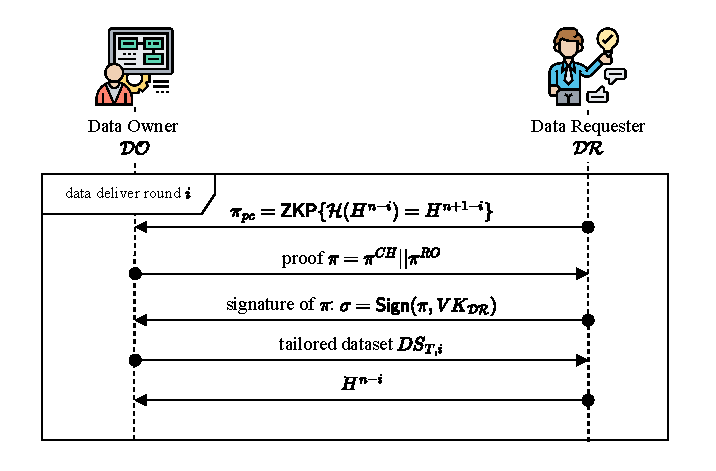
\includegraphics[width=1.0\linewidth]{figures/scheme/data-delivery.pdf}
    \caption{Data Delivery Process}\label{fig:data_delivery}
\end{figure}
In data trading ecosystems, achieving fair exchange between $\mathcal{DO}$ and $\mathcal{DR}$ presents significant challenges.  Key challenges include: 1) ensuring data meets specified constraints before payment, 2) preventing either party from abandoning the exchange after receiving their desired asset, and 3) resolving disputes without revealing sensitive data to external validators. To address these challenges, we propose a multi-round fair exchange protocol that divides the tailored dataset into multiple subsets and employs a gradual delivery mechanism with cryptographic commitments. This approach balances security and efficiency by limiting potential losses from malicious behavior while providing on-chain dispute resolution that preserves data privacy. 

After generating a tailored dataset $DS_T$ according to data request $R$ (for instance, $DS_T$ is generated from $DS_{IV}$ as shown in Fig.~\ref{fig:IMT}), $\mathcal{DO}$ divides $DS_T$ into $n $ subsets, denoted as $DS_{T,1}, DS_{T,2},...,DS_{T,n}$, and generates relevant proofs for each subset. After generating valid proofs for $DS_{T,1}, DS_{T,2},...,DS_{T,n}$, $\mathcal{DO}$ and $\mathcal{DR}$ engage in multi-round data delivery process to exchange a tailored dataset and a payment commitment. Each round consists of five steps of interactions. Fig.~\ref{fig:data_delivery} illustrates the process flow of the $i$-th round.
\begin{enumerate}
    \item $\mathcal{DR} \rightarrow \mathcal{DO}$: validity proof of payment commitment $\pi_{pc}$.
    
    To prevent $\mathcal{DO}$ from refusing to deliver tailored dataset or provide invalid tailored dataset after receiving a valid plaintext payment commitment from $\mathcal{DR}$ at the last loop, thereby obtaining an extra undeserved fund, $\mathcal{DR}$ only provides the validity proof of the payment commitment in the first round. $\pi_{pc} = \mathsf{ZKP}\{H^{(n-i)},H^{(n+1-i)} : \mathcal{H}(H^{(n-i)}) = H^{(n+1-i)}\}$,  where $H^{(n-i)}$ is the private input and $H^{(n+1-i)}$ is the public input of proof.
    
    \item $\mathcal{DO} \rightarrow \mathcal{DR}$: zk-SNARK proof of tailored dataset.
    
    To prevent $\mathcal{DR}$ from refusing to provide valid payment commitment after receiving the tailored dataset, $\mathcal{DO}$ only delivers the proof of $DS_{T,i}$ without providing the $DS_{T,i}$ itself. $\pi = \pi^{CH} || \pi^{RO}$. 
    For the customized dataset $DS_{T,i}$, which contains both masked data and plaintext data, different verification mechanisms are applied. For masked data, the combination of corresponding $\pi^{CH}$ and $\pi^{RO}$ can prove both the validity of constraints and data integrity. For plaintext data, the corresponding $\pi^{RO}$ can prove that if its hash value is $h$, then $h$ must exist as a leaf node in the $\mathsf{IMT}$ of the $\mathsf{DC}$. However, due to zero knowledge property of zk-SNARK for private inputs, when the $\mathcal{DR}$ only obtains the proof $\pi$ without access to the plaintext content of the $DS_{T,i}$, he/she can only verify the existence of the data.  $\mathcal{DR}$ cannot determine the validity of constraints for plaintext data and whether its hash value is indeed $h$.
    
    \item $\mathcal{DR} \rightarrow \mathcal{DO}$: signature of proof $\pi$.

    If the proof $\pi$ is valid, $\mathcal{DR}$ sends $\mathcal{DO}$ a signature $\sigma = \mathsf{Sign}\{vk_{DR}, \mathcal{H}(\pi)\}$ of proof $\pi$ to indicate agreement with the current round, and request that this loop should continue. If the proof $\pi$ is invalid, $\mathcal{DR}$ can invoke the $\mathsf{VC}$ to deduct the deposit of $\mathcal{DO}$.

    \item $\mathcal{DO} \rightarrow \mathcal{DR}$: tailored dataset $DS_{T,i}$.

    To prevent $\mathcal{DR}$ from falsely claiming that it did not receive the tailored dataset and refusing to provide valid payment commitment, $\mathcal{DO}$ only provide the $DS_{T,i}$ after receiving $\mathcal{DR}$'s valid signature of proof $\pi$. After receiving the tailored dataset, $\mathcal{DR}$ can verify the validity of constraints and integrity of plaintext data. If any constraint violation or integrity mismatch is detected, $\mathcal{DR}$ can submit evidence to the verification contract  to deduct the deposit from $\mathcal{DO}$.

    \item $\mathcal{DR} \rightarrow \mathcal{DO}$: payment commitment.
    If the plaintext part of tailored dataset still satisfies the constraints and the integrity is valid, $\mathcal{DR}$ will provide the valid payment commitment $H^{n-i}$. If $\mathcal{DR}$ still refuses to provide $H^{i-1}$, $\mathcal{DO}$ can submit evidence on verification contract to appeal for the fund of this round. 
\end{enumerate}

\textbf{Dispute Resolve}
Here we discuss the case of dispute resolution details between $\mathcal{DO}$ and $\mathcal{DR}$, where one may believe that the other one acts in malicious manner.
\begin{itemize}
    \item \textbf{Invalid zk-SNARK proof}. If $\mathcal{DR}$ believes that $\mathcal{DO}$ sends an invalid proof $\pi$ in step 2, $\mathcal{DR}$ can submit the evidence, the specific invalid proof $\pi^{CH}$ or $\pi^{RO}$, to the $\mathsf{VC}$. If $\mathsf{VC}$ verify that the proof is invalid indeed, $\mathsf{VC}$ will deduct the deposit of $\mathcal{DO}$ and transfer to $\mathcal{DR}$ and terminate this delivery process.
    \item \textbf{Invalid plaintext data}. If $\mathcal{DR}$ believes that $\mathcal{DO}$ sends invalid plaintext data in step 4, including data that fails to meet the plaintext data constraints or the hash of data does not match with hash in corresponding $\pi^{RO}$, $\mathcal{DR}$ can submit evidence to $\mathsf{VC}$. Once $\mathsf{VC}$ confirms that the data violates the constraints or the hash does not match, it will deduct $\mathcal{DO}$'s deposit to $\mathcal{DR}$ and terminate the delivery process.
    \item \textbf{Claim reward of the last round}. If $\mathcal{DO}$ provides valid tailored dataset in step 5, but $\mathcal{DR}$ does not to send the payment commitment $H^{n-i}$ in step 6, $\mathcal{DO}$ can submit evidence to $\mathsf{VC}$ to claim the reward for this round. The evidence should include the payment commitment proof $\pi_{pc}$ for the current round, the signature of proof $\sigma$, and the plaintext of the tailored dataset $DS_{T,i}$. If $VC$ verifies that all constraints are satisfied and integrity is guaranteed, it will transfer the fund for this round to $\mathcal{DO}$.  Note that even if $\mathcal{DO}$ attempts to act maliciously by not delivering the dataset after receiving the signature and directly claiming the reward through $\mathsf{VC}$, this strategy would be counterproductive. This is because claiming through $\mathsf{VC}$ requires $\mathcal{DO}$ to publicly submit the dataset and pay additional transaction fees, while $\mathcal{DR}$ would still obtain the dataset, resulting in $\mathcal{DO}$ only receiving the deserved payment for this round minus extra transaction costs.
\end{itemize}

\subsection{Data Trading Process}\label{subsec:data_delivery_verfication}

Our complete data trading scheme consists of four sequential phases that collectively enable secure, verifiable, and fair exchange of customized data between data owners and requesters. This section provides the detail of the entire trading process.

\textbf{1) Data Upload}. $\mathcal{DO}$ collects valuable datasets through various devices or systems. Upon collecting sufficient data, $\mathcal{DO}$ constructs the integrity Merkle tree $\mathsf{IMT}$ by first hashing individual field values with random salts at the entry layer, then building dataset-level trees that combine attribute and entry subtrees, followed by aggregating multiple datasets, and finally applying padding to reach the maximum depth $D_{max}$. After completing the $\mathsf{IMT}$ construction, $\mathcal{DO}$ deploys a data contract $\mathsf{DC}$ on the blockchain, uploading only the root hash $R$ of the $\mathsf{IMT}$ along with comprehensive data descriptions including available attributes, entry fields, data collection periods, and general characteristics. $\mathsf{DC}$ serves as a verifiable commitment to the dataset's integrity and enables subsequent proof verification during the trading process.

\begin{figure}[htbp]
    \centering
    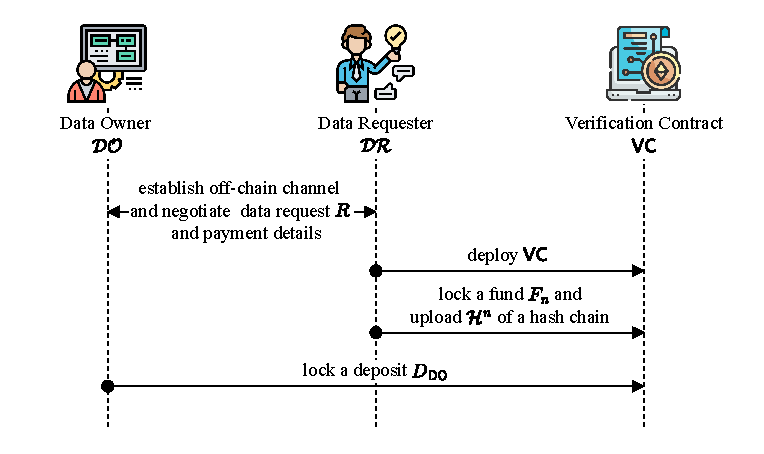
\includegraphics[width=1.0\linewidth]{figures/scheme/data-request.pdf}
    \caption{Data Request Process}\label{fig:data_request}
\end{figure}
\textbf{2) Data Request}. After retrieving data description from data contract on blockchain, $\mathcal{DR}$ selects a suitable $\mathcal{DO}$ based on their requirements and start the data request process which consists of off-chain parts and on-chain parts.
In the off-chain parts, $\mathcal{DR}$ and $\mathcal{DO}$ establish an off-chain channel and negotiate about the trading details including data request $R$ and payment details, such as the number of data entries per transaction round, the transaction fund for each round and the estimated total number of transaction rounds. Once $\mathcal{DO}$ and $\mathcal{DR}$ reach consensus on transaction details, they proceed to on-chain phase. 
In the on-chain part, $\mathcal{DR}$ deploys a verification contract, denoted as $\mathsf{VC}$ on the blockchain after a successful negotiation. The $\mathsf{VC}$ deploys a plaintext constraint verification function, a constraint-hash proof verification function, a root obfuscation proof verification function, a signature verification function in addition to the fund management process.
Then $\mathcal{DR}$ locks a certain amount of funds $F_n$ and uploads the anchor of a hash chain $\mathcal{H}^{(n)}$ by selecting a secret value $s$ and recursively applying the hash function $n$ times: $\mathcal{H}^{(n)}(s)=H^{(n)}$. $\mathcal{DO}$ then locks a security deposit $D_{DO}$ on $\mathsf{VC}$. If $\mathcal{DR}$ can invoke the verification function to prove that $\mathcal{DO}$ give invalid dataset, then the deposit $D_{DO}$ will be transferred to $\mathcal{DR}$.  

\textbf{3) Data Delivery and Verification}. 
After the verification contract $\mathsf{VC}$ is deployed with both parties' funds locked, $\mathcal{DO}$ and $\mathcal{DR}$ proceed with the multi-round data delivery protocol. $\mathcal{DO}$ package a tailored dataset $DS_T$ that satisfies request $R$ by filtering and masking the original dataset $DS$. The tailored dataset maintains the binary structure like the original dataset $DS_T = \{A_T, E_T\}$, where $A_T$ and $E_T$ are the processed attribute set and entry set respectively. $A_T$ contains all key-value pairs covered by the attribute request in data request $R$:
$A_T = \{(k_i, v'_i) | 1\leq i \leq p,k_i \in K_{R_a^p} \cup K_{R_a^{m}}, v'_i = \begin{cases} v_i & \text{if } k_i \in K_{R_a^p} \land v_i \models c_i^a \\ mr_i(v_i) & \text{if } k_i \in K_{R_a^m} \land v_i \models c_i^a\end{cases}\}$. For keys $k_i \in K_{R_a^p}$ in plaintext attribute requests, if the original value $v_i$ satisfies the constraint condition $c_i$, it is retained directly. For keys $k_i \in K_{R_a^m}$ in masking attribute requests, if the original value $v_i$ satisfies the constraint condition $c_i$, it is retained after applying the masking rule $mr_i$. $E_T$ contains processed data entries that satisfy the conditions: 
$E_T = \{e_i^T = (e_i^{f_1}, e_i^{f_2}, ..., e_i^{f_t}) |1 \leq i \leq q, 1 \leq j \leq t, e_i^{f_j} = \begin{cases}e_i^{f_j} & \text{if } f_j \in F_{R_e^p} \land e_i^{f_j} \models c_j^f \\mr_j(e_i^{f_j}) & \text{if } f_j \in F_{R_e^m} \land e_i^{f_j} \models c_j^f\end{cases}\}$. For fields $f_j \in F_{R_e^p}$ in plaintext field requests, if the original value $e_i^{f_j}$ satisfies the constraint condition $c_j$, it is retained directly. For fields $f_j \in F_{R_e^m}$ in masking field requests, if the original value $e_i^{f_j}$ satisfies the constraint condition $c_j$, it is retained after applying the masking rule $mr_j$. An entry $e_i$ is retained in $E_T$ only when all its requested fields satisfy their corresponding constraint conditions. 

The tailored dataset $DS_T$ is divided into $n$ subsets, and each subset is exchanged following the five-step protocol described in Section~\ref{fig:data_delivery}. For each round $i$, $\mathcal{DR}$ first provides proof of payment commitment validity. Upon verification, $\mathcal{DO}$ delivers zero-knowledge proofs demonstrating both constraint satisfaction and data integrity of subset $DS_{T,i}$. After $\mathcal{DR}$ verifies and signs these proofs, $\mathcal{DO}$ releases the actual data subset. Finally, if the received data is valid, $\mathcal{DR}$ reveals the corresponding payment commitment pre-image. If disputes arise during any round, either party can invoke the verification functions in $\mathsf{VC}$ to resolve conflicts. The dispute resolution mechanisms handle cases of invalid proofs, constraint violations, or payment refusals without requiring trusted third parties.

\textbf{4) Payment Settlement}.
The final phase of our trading scheme handles the settlement of all outstanding payments and the release of remaining funds to their rightful owners. After the off-chain multi-round delivery process concludes, whether through completion of all planned rounds or early termination due to disputes, $\mathcal{DO}$ initiates the settlement process by submitting the latest payment commitment pre-image $H^m$ to the verification contract $\mathsf{VC}$. This submission represents a claim for payment corresponding to $n-m$ successfully completed data delivery rounds, where $n$ represents the total initial rounds and $m$ represents the remaining unrevealed commitments. The smart contract performs automated verification by computing the hash chain validation: $\mathcal{H}^{(n-m)}(H^m) = H^{(n)}$, where $\mathcal{H}^{(n-m)}$ denotes applying the hash function $n-m$ times iteratively. This cryptographic verification ensures that $\mathcal{DO}$ legitimately earned the claimed payment through valid data deliveries, as each revealed pre-image corresponds to one successfully completed trading round. Upon successful verification, the smart contract automatically transfers the corresponding reward amount of $(n-m) \times b$ to the designated address of the data owner ($\mathcal{DO}$), as compensation for all delivered data subsets. Here, $b$ represents the pre-negotiated price per data subset established during the data request phase. Simultaneously, the contract releases the remaining locked funds $m \times b$ back to $\mathcal{DR}$, representing payment for trading rounds that were never completed or were terminated due to disputes. Additionally, $\mathcal{DO}$'s security deposit $D_{DO}$ is returned unless it was previously forfeited due to proven malicious behavior during the delivery process. This automated settlement mechanism ensures precise payment allocation based on actual data delivery performance while eliminating the need for manual intervention or trusted third-party arbitration.

\section{Security analysis }\label{section:security_analysis}

In this section, we analyze the security properties of our scheme, focusing on data privacy preservation, verifiability of masked data constraint and integrity, and data delivery fairness.

\subsection{Data Privacy Preservation}
Based on the fundamental zero-knowledge property of zk-SNARKs, we demonstrate that our design goal of ``Data Privacy Preservation" is achieved through two complementary security properties: ``Sensitive Information Confidentiality" and ``Data Scale and Structure Confidentiality".

\begin{lemma}[Zero-Knowledge Property of zk-SNARK]
\label{lemma:zk-snark-property}
Since zk-SNARK inherently possesses the zero-knowledge property, there exists a polynomial-time simulator $\mathcal{S}_{zk}$ capable of generating a simulated zk-SNARK proof $\tilde{\pi}_{zk}$ without using the actual sensitive input. Consequently, for any polynomial-time adversary $\mathcal{A}$, it holds that $\Pr[\mathcal{A}(\pi_{zk}) = 1] \approx \Pr[\mathcal{A}(\tilde{\pi}_{zk}) = 1]$.
\end{lemma}

\begin{theorem}
\textbf{Sensitive Information Confidentiality.}
\label{theorem:sensitive-confidentiality}
The constraint-hash proof $\pi_{a}^{CH}$ and $\pi_{e}^{CH}$ ensure that no information about the sensitive values $v_i$ and $e_j^{f_t}$ is leaked beyond what is implied by their hash values $h_i$ and $h_j^{f_t}$.
\end{theorem}

\begin{proof}
We prove this by constructing a simulator for each proof type. For $\pi_{a}^{CH}(v_i)$, by Lemma~\ref{lemma:zk-snark-property}, there exists a simulator $\mathcal{S}_a$ that can generate a simulated proof $\tilde{\pi}_{a}^{CH}$ given only the public input $h_i$, such that $\tilde{\pi}_{a}^{CH}$ is computationally indistinguishable from a real proof $\pi_{a}^{CH}(v_i)$ generated using the actual attribute value $v_i$. Similarly, for $\pi_{e}^{CH}(e_j^{f_t})$, there exists a simulator $\mathcal{S}_e$ that can generate a simulated proof $\tilde{\pi}_{e}^{CH}$ given only the public input $h_j^{f_t}$, such that $\tilde{\pi}_{e}^{CH}$ is computationally indistinguishable from a real proof $\pi_{e}^{CH}(e_j^{f_t})$ generated using the actual field value $e_j^{f_t}$.
Since the simulators can generate indistinguishable proofs without access to the sensitive values, the proofs themselves cannot reveal any additional information about these values beyond what is already known from the hash values. The hash function $\mathcal{H}$ is assumed to be preimage-resistant, ensuring that the hash values themselves do not leak information about the original values. Therefore, the constraint-hash proofs preserve the confidentiality of sensitive attribute and field values.
\end{proof}

\begin{theorem}
\textbf{Data Scale and Structure Confidentiality.}
\label{theorem:scale-confidentiality}
The root obfuscation proof $\pi_{h}^{RO}$ ensures that no information about the data scale, batch organization, or hierarchical structure is leaked beyond what is implied by the root list $RL$.
\end{theorem}

\begin{proof}
The root obfuscation proof $\pi_{h}^{RO}$ takes the Merkle proof $MP(h)$ and the index $i$ as private inputs, with only the root list $RL$ being public. By Lemma~\ref{lemma:zk-snark-property}, there exists a simulator $\mathcal{S}_h$ that can generate a simulated proof $\tilde{\pi}_{h}^{RO}$ given only the public input $RL$, such that $\tilde{\pi}_{h}^{RO}$ is computationally indistinguishable from a real proof $\pi_{h}^{RO}$ generated using the actual Merkle proof $MP(h)$ and index $i$.
Since the simulator can generate an indistinguishable proof without knowledge of:
\begin{itemize}
    \item The specific Merkle proof path $MP(h)$, which would reveal the depth and structure of the tree.
    \item The specific index $i$ of the root in $RL$, which would reveal which data batch the value belongs to.
    \item The specific leaf position within the tree, which is concealed by the padding layer of the $\mathsf{IMT}$.
\end{itemize}
The proof itself cannot reveal any additional information about the data scale, batch organization, or hierarchical structure beyond what is already known from the root list $RL$. The padding mechanism in the $\mathsf{IMT}$ further obfuscates the actual data scale by introducing dummy nodes. Furthermore, the collision resistance property of the hash function used in the $\mathsf{IMT}$ construction ensures that an adversary cannot find alternative data structures that would map to the same root values in $RL$, thereby preserving the integrity of the concealed data organization. Therefore, the root obfuscation proof preserves the confidentiality of data scale and organizational structure.
\end{proof}

\subsection{Verifiability of Constraint Validity and Data Integrity}
We first present two lemmas: the completeness and soundness of zk-SNARKs. Based on these fundamental properties, we can establish that our design goal of ``Verifiability of Constraint Validity and Data Integrity" is achievable as long as the $\mathcal{DO}$ has the valid data that can satisfy the constraints and generate valid merkle proofs. Then the verifiability is supported by two key security properties: Constraint Unforgeability and Data Immutability, which we prove in the following theorems.

\begin{lemma} \label{lemma:completeness}
    \textbf{(Completeness of zk-SNARK)} 
    For any statement $x$ in the language $L$ with a valid witness $w$, an honest prover can always generate a proof $\pi$ that convinces an honest verifier with probability 1, i.e.,
    \begin{equation}
        \forall (x, w) \in R_L: \Pr[\text{Verify}(vk, x, \text{Prove}(pk, x, w)) = 1] = 1
    \end{equation}
    where $R_L$ is the relation defining language $L$, $pk$ is the proving key, and $vk$ is the verification key.
\end{lemma}

\begin{lemma} \label{lemma:soundness}
    \textbf{(Soundness of zk-SNARK)} 
    For any computationally bounded adversary $\mathcal{A}$, the probability of generating a valid proof for a statement not in the language $L$ is negligible, i.e.,
    \begin{equation}
        \forall x \notin L, \forall \mathcal{A}: \Pr[\text{Verify}(vk, x, \mathcal{A}(pk, x)) = 1] \leq \text{negl}(\lambda)
    \end{equation}
    where $\lambda$ is the security parameter, and $\text{negl}(\lambda)$ is a negligible function in $\lambda$.
\end{lemma}
\begin{theorem}
    \textbf{(Constraint Unforgeability)} 
     Let $R=\{R_a,R_e\}$ be a data request with constraint conditions $c_i^a$ for attributes and $c_j^f$ for entry fields. A computationally bounded adversary $\mathcal{A}$ cannot generate valid constraint-hash proofs for data that does not satisfy the specified constraints, except with negligible probability.
\end{theorem}

\begin{proof}
    Consider an adversary $\mathcal{A}$ who possesses data that does not satisfy the specified constraints. Specifically, let $v_i$ be an attribute value that does not satisfy constraint $c_i^a$ (i.e., $v_i \not\models c_i^a$), and let $h_i = \mathcal{H}(v_i)$. For $\mathcal{A}$ to successfully forge a valid constraint-hash proof, $\mathcal{A}$ must generate a proof $\pi'$ such that:
    $$
        \text{Verify}(vk, (c_i^a, h_i), \pi') = 1
    $$
    However, the statement ``there exists a value that satisfies $c_i^a$ and hashes to $h_i$" is false because:
    \begin{itemize}
        \item $v_i$ does not satisfy $c_i^a$ by assumption.
        \item Due to the collision resistance of the hash function $\mathcal{H}$, finding another value $v_i'$ such that $v_i' \models c_i^a$ and $\mathcal{H}(v_i') = h_i$ is computationally infeasible.
    \end{itemize}
    By Lemma \ref{lemma:soundness} (ZK-SNARK Soundness), for any proof $\pi'$ that $\mathcal{A}$ might generate:
    $$
        \Pr[\text{Verify}(vk, (c_i^a, h_i), \pi') = 1] \leq \text{negl}(\lambda)
    $$
    The same argument applies to entry field values that do not satisfy their respective constraints. Therefore, an adversary cannot generate valid constraint-hash proofs for data that violates the specified constraints, except with negligible probability. Conversely, by Lemma \ref{lemma:completeness} (ZK-SNARK Completeness), an honest data owner $\mathcal{DO}$ who possesses data satisfying all constraints can always generate valid proofs that will be accepted by the data requester $\mathcal{DR}$ with probability 1. Thus, the constraint-hash proof mechanism ensures that only data satisfying the specified constraints can be proven valid, establishing the unforgeability of constraint validation.
\end{proof}

\begin{theorem}
    \textbf{(Data Immutability)} 
    Let $\mathcal{H}$ be a collision-resistant hash function. Consider the Merkle Trees $\mathsf{IMT}$ constructed using $\mathcal{H}$. For any data entry $d$, a computationally bounded adversary $\mathcal{A}$ cannot modify $d$ to $d'$ and generate valid proofs corresponding to $d'$ except with negligible probability.
\end{theorem}

\begin{proof}
    We prove the theorem by contradiction. Assume that an adversary $\mathcal{A}$ who, in polynomial time, successfully generates valid proofs $\pi' = \pi^{CH} || \pi^{RO}$ for the tampered data entry $d'$. Let the original data entry $d_0$ be composed of two parts: attribute information $d_0^{attr}$ and structured relationship data $d_0^{set}$, such that $d_0 = \{d_0^{a} \parallel d_0^{e}\}$.
    We examine the possible cases where $\mathcal{A}$ modifies $d_0$ to $d'_0$:
    \begin{itemize}
        \item \textbf{Case 1}: $\mathcal{A}$ modifies $d^{a}_0$ to $d'^{a}_0$ but generates valid constraint-hash proof $\pi^{CH}_a$ that includes the circuits verifying $h = \mathcal{H}(d'^{a}_0)$. 

        \item \textbf{Case 2}: $\mathcal{A}$ modifies $d^{e}_0$ to $d'^{e}_0$ but generates valid constraint-hash proof $\pi^{CH}_e$ that includes the circuits verifying $h = \mathcal{H}(d'^{e}_0)$.
    
        \item \textbf{Case 3}: $\mathcal{A}$ modifies $d^{a}_0$ to $d'^{a}_0$ and generates $\pi'^{CH}_a$ that includes the circuits verifying $\mathcal{H}(d'^{e}_0) = h'$. A root obfuscation proof $\pi^{RO}_{h'}$ is generated for $h'$.

        \item \textbf{Case 4}: $\mathcal{A}$ modifies $d^{e}_0$ to $d'^{e}_0$ and generates $\pi'^{CH}_e$ that includes the circuits that $\mathcal{H}(d'^{e}_0) = h'$. A root obfuscation proof $\pi^{RO}_{h'}$ is generated for $h'$.

    \end{itemize}
    In both Case 1 and Case 2, the situations are similar. $\mathcal{A}$ needs to generate a valid hash proof for the altered data $d'$ to demonstrate that $\mathcal{H}(d') = \mathcal{H}(d) = h$. This requirement contradicts the second pre-image resistance property of hash functions. Similarly, in Case 3 and Case 4, $\mathcal{A}$ must produce a valid Merkle proof for the new hash value $h'$. Given the collision resistance of hash functions, this task becomes even more improbable.
\end{proof}

\subsection{Data Delivery Fairness}
\begin{theorem}
    \textbf{(Fair Guarantee)} 
    Assuming the security of digital signatures and zk-SNARK systems, in the data delivery protocol, the following properties are guaranteed:
    \begin{itemize}
        \item $\mathcal{DO}$ cannot obtain payment without delivering valid data.
        \item $\mathcal{DR}$ cannot obtain valid data without making payment.
    \end{itemize}
\end{theorem}

\begin{proof}
    We prove this by analyzing possible deviation strategies of both parties and showing none can succeed. First, consider possible malicious strategies by $\mathcal{DO}$:
    \begin{itemize}
        \item \textbf{Case 1}: $\mathcal{DO}$ tries to obtain payment by providing invalid proof $\pi$ in Step 2. In this case, $\mathcal{DR}$ can detect the invalid proof and refuse to provide signature $\sigma$. Furthermore, $\mathcal{DR}$ can submit evidence to $\mathsf{VC}$ to claim $\mathcal{DO}$'s deposit.
        
        \item \textbf{Case 2}: $\mathcal{DO}$ provides valid proof $\pi$ but invalid dataset $DS_{T,i}$ in Step 4. After receiving invalid data, $\mathcal{DR}$ can verify and detect violations in plaintext constraints or data integrity. $\mathcal{DR}$ can then submit evidence to $\mathsf{VC}$ to claim $\mathcal{DO}$'s deposit.

        \item \textbf{Case 3}: $\mathcal{DO}$ tries to claim payment through $\mathsf{VC}$ without delivering data. To claim payment, $\mathcal{DO}$ must submit the actual dataset to $\mathsf{VC}$, which means $\mathcal{DR}$ still obtains the data while $\mathcal{DO}$ incurs extra transaction fees.
    \end{itemize}
    Next, consider possible malicious strategies by $\mathcal{DR}$:
    \begin{itemize}
        \item \textbf{Case 1}: $\mathcal{DR}$ provides invalid payment commitment proof $\pi_{pc}$ in Step 1. $\mathcal{DO}$ can detect this immediately and refuse to continue the protocol.

        \item \textbf{Case 2}: $\mathcal{DR}$ tries to obtain data without providing valid signature in Step 3. Without valid signature $\sigma$, $\mathcal{DO}$ will not proceed to deliver the actual dataset.

        \item \textbf{Case 3}: $\mathcal{DR}$ refuses to provide payment commitment after receiving valid data. $\mathcal{DO}$ can submit evidence including $\pi_{pc}$, $\pi$, $\sigma$, and $DS_{T,i}$ to $\mathsf{VC}$ to claim payment.
    \end{itemize}
    In summary, any deviation from the protocol by either party will result in either:
    \begin{itemize}
        \item Protocol termination before any exchange occurs.
        \item The malicious $\mathcal{DO}$ losing his/her deposit.
        \item The honest party still receiving their entitled assets (data or payment).
    \end{itemize}
    This proves that the protocol ensures fair exchange of data and payment between both parties.
\end{proof}

\section{Performance Analysis}\label{section:performance_analysis}
In this section, we conduct a comprehensive performance evaluation of two crucial components in our scheme: the efficiency of zk-SNARK proof generation and verification, and the actual economical cost on Ethereum. For the zk-SNARK proof component, we use gnark\cite{gnark} and gnark-crypto\cite{gnark-crypto} for basic proof generation in Section \ref{subsec:data_delivery_verfication}. Regarding on-chain costs, we implement smart contracts in our scheme in Solidity and conduct cost analyses at various stages on both Ethereum Sepolia and zkSync Sepolia test networks by foundry\cite{foundry}. The experimental results strongly demonstrates the efficiency and economic viability of our proposed scheme.

\subsection{ Performance of zk-SNARK Proof}

We implement the corresponding circuit using gnark\cite{gnark} and gnark-crypto\cite{gnark-crypto}. Gnark supports two prominent zk-SNARK protocols: Groth16\cite{groth2016size} and Plonk\cite{gabizon2019Plonk}. Our scheme requires the verification of zk-SNARK proofs within Ethereum smart contracts. Currently, Ethereum only natively supports the BN254 elliptic curve through its precompiled contracts. Therefore, we choose to generate and verify all zk-SNARK proofs on BN254. This curve offers approximately 128 bits of security, which is sufficient to meet the security requirements of our current application scenario.



The experiments for generating and verifying our zk-SNARK proofs are conducted on a server equipped with two Intel(R) Xeon(R) Gold 6330 CPUs running at 2.00GHz and 256GB of memory. The server runs Ubuntu 22.04 LTS with Linux kernel 5.15.0-101-generic. 

As mentioned in Section~\ref{subsec:data_delivery_verfication}, there are two types of proofs based on zk-SNARK: one is constraint-hash proof, and the other is the root obfuscation proof. We present the proof generation and verification time to demonstrate the efficiency of zk-SNARK in our scheme.
\subsubsection{Constraint-Hash Proof}
To evaluate the efficiency of our constraint-based hash proof system, we conducted experimental assessments on three distinct constraint types: range constraints, subset constraints, and substring (substr) constraints. 
The range-hash proof demonstrates that a preimage falls within a specified interval $[min, max]$ and yields a hash value $H$, without revealing the actual preimage content. The subset-hash proof verifies that a preimage corresponds to an element from a predefined set containing multiple hash values. The substr-hash proof involves disclosing a portion of the preimage while providing hash verification for the complete preimage. Considering the performance requirements for hash functions in practical applications, we select MiMC\cite{albrecht2016mimc} in gnark-crypto as the hash function in zk-SNARK circuits.
We conducted performance tests for proof generation and verification on each of the three constraints, and the experimental results are illustrated in the accompanying figures.

\begin{figure}[htbp]
    \centering
    \subfigure[Proof Generation Time with Different Constraint ]{
        \label{fig_constraint_hash_prove}
        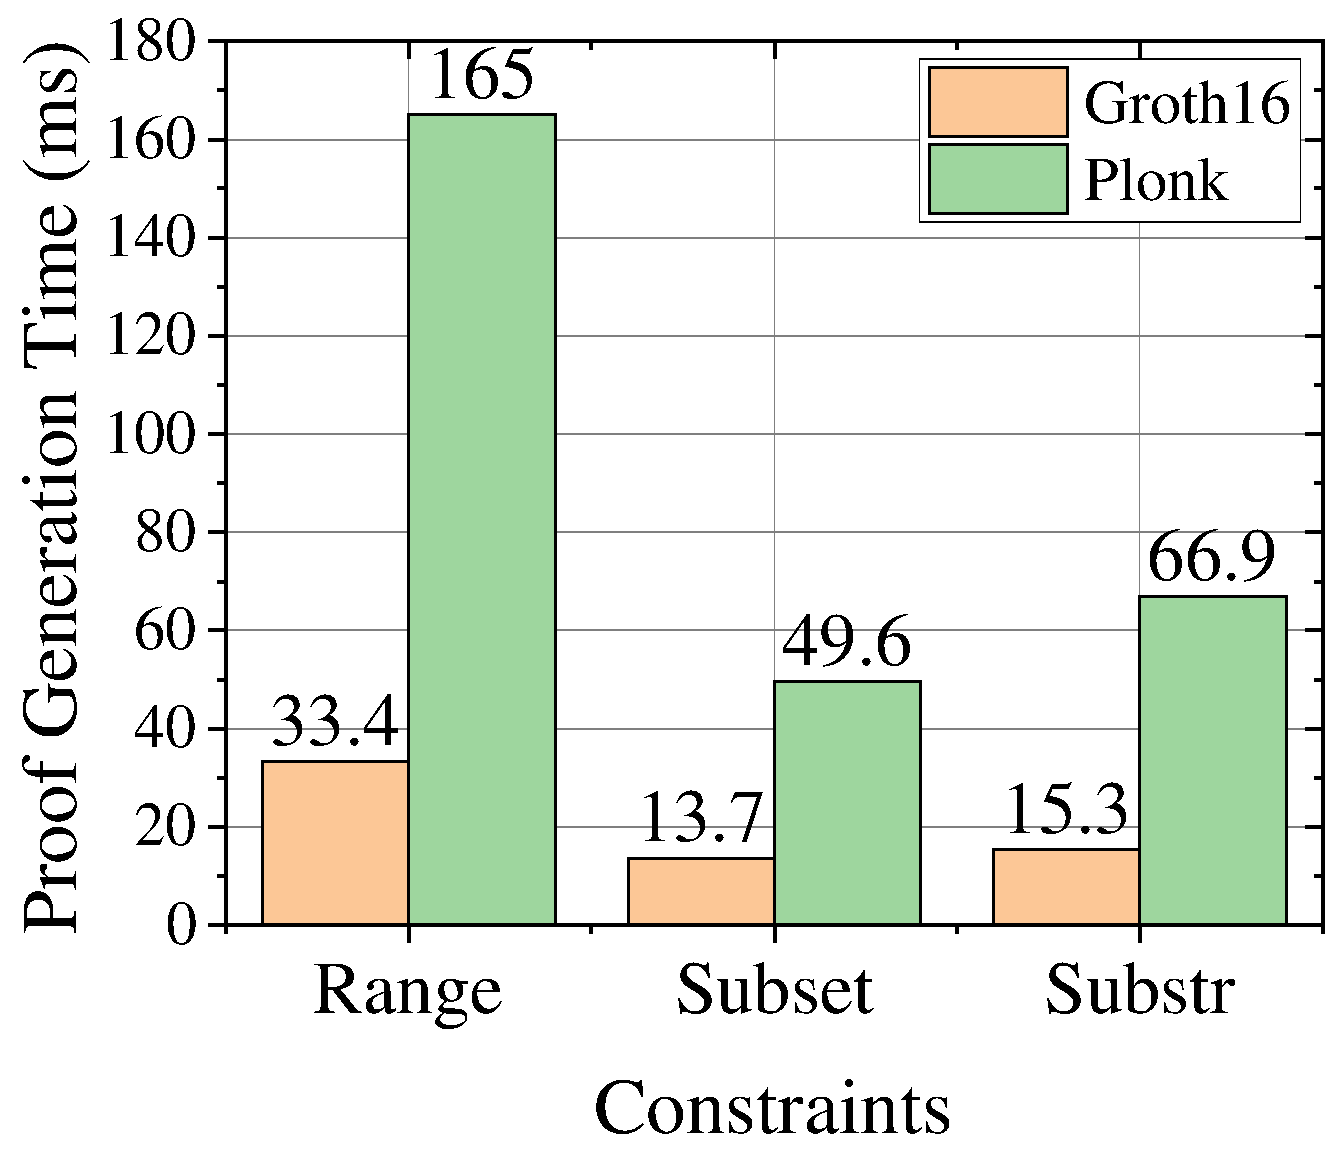
\includegraphics[width=0.45\linewidth]{figures/exp/constraint_hash_prove_time.pdf}
    }
    \subfigure[Number of \emph{Circuit} Constraints with Different Constraints]{
        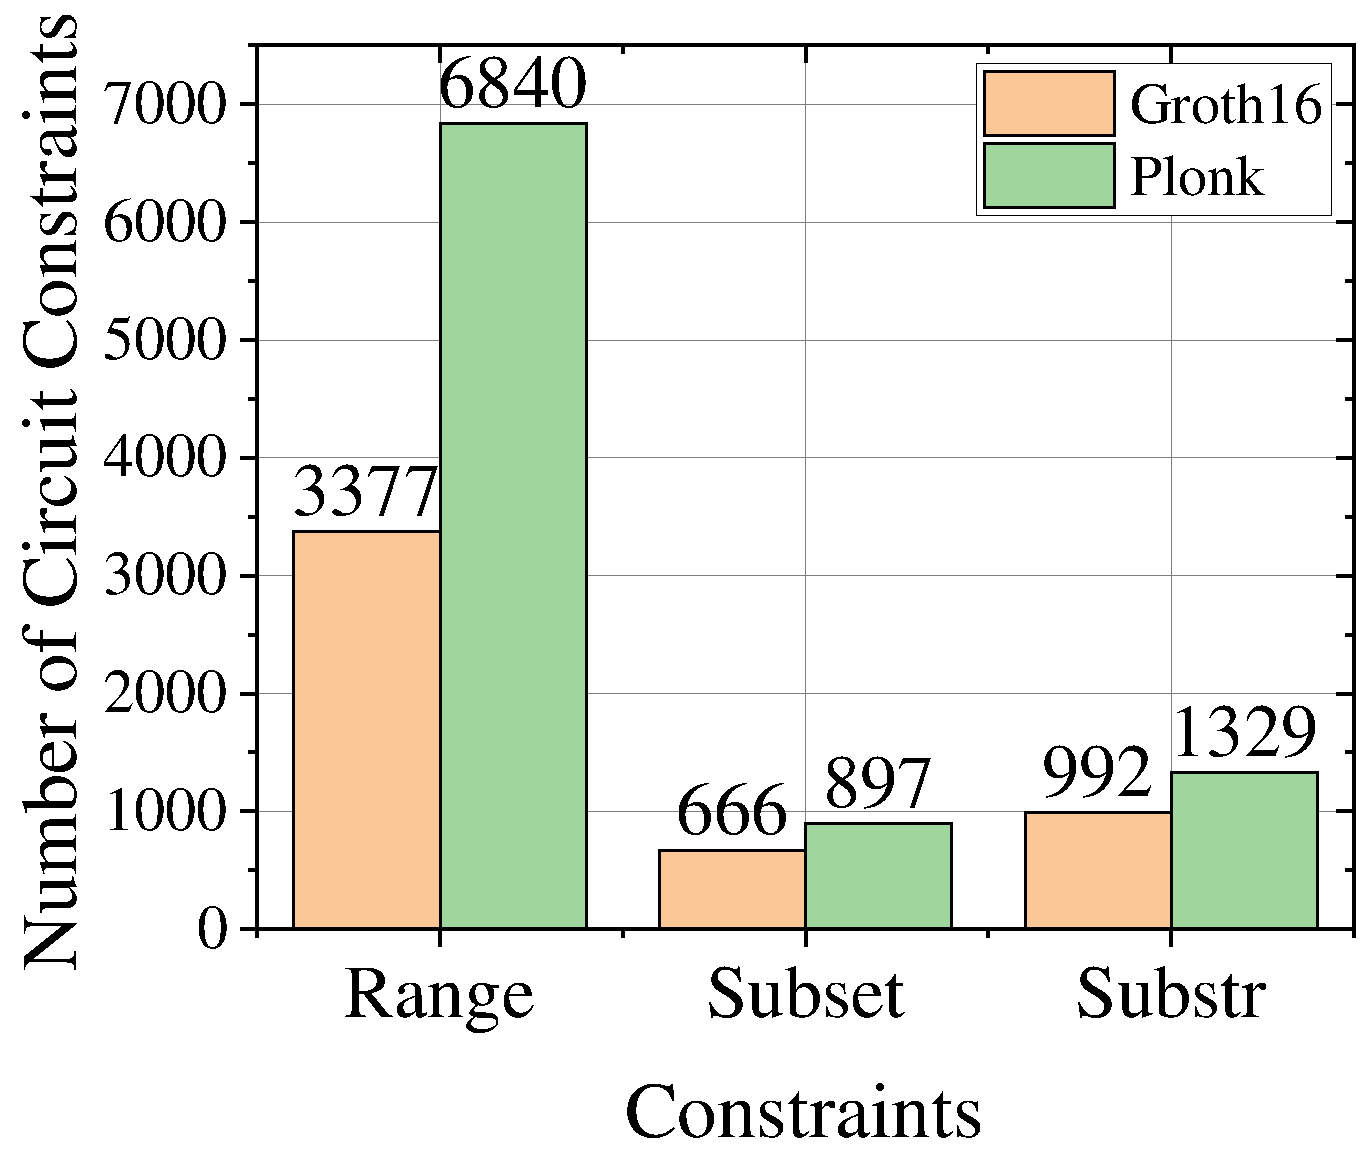
\includegraphics[width=0.45\linewidth]{figures/exp/constraint_hash_constraints_num.pdf}
        \label{fig_constraint_hash_constraints}
    }
    \caption{Performance of Constraint-hash Proof Generation}
    \label{fig_constraint_hash}
\end{figure}
Fig.~\ref{fig_constraint_hash_prove} illustrates the proof generation time under different constraint for both Groth16 and Plonk zero-knowledge proof protocols. Fig.~\ref{fig_constraint_hash_constraints} presents the corresponding number of \emph{circuit} constraints (different from the constraints we want to prove) included in each proof. The analysis reveals that under identical constraint, Groth16 protocol requires significantly fewer \emph{circuit} constraints compared to Plonk, thus achieving higher computational efficiency. Notably, in the case of constraint-hash proof, the proof generation time remains under 40 milliseconds, demonstrating exceptional performance characteristics.

\begin{table*}[htbp]
    \centering
    % \linespread{1.3}\selectfont
    \caption{On-chain Costs }
    \label{tab_gas_cost}
    \begin{tabular}{c|c|c|c|c}
    \hline
    % \hline
    Scenarios   & Sepolia Gas Cost & Sepolia Eth Cost & Zksync Sepolia Gas Cost & Zksync Sepolia Eth Cost \\
    \hline 

    $\mathcal{DR}$ Deploy Contracts & 10822935 & 0.0148 & 114897714 & 0.0114 \\

    $\mathcal{DO}$ Lock Deposit & 75808 & 0.000104 & 487377 & 0.0000487 \\

    $\mathcal{DO}$ Fund Claim & 95596 & 0.000131 & 824257 & 0.0000824 \\
      
    $\mathcal{DR}$ Punish $\mathcal{DO}$ for Invalid range-hash proof   & 314897 & 0.000432 & 9436197 & 0.000943 \\ 
    $\mathcal{DR}$ Punish $\mathcal{DO}$ for Invalid subset-hash proof   & 114019 & 0.000156 & 526542 & 0.0000526 \\ 
    $\mathcal{DR}$ Punish $\mathcal{DO}$ for Invalid substr-hash proof   & 307858 & 0.000422 & 9278704 & 0.000927 \\ 

    $\mathcal{DR}$ Punish $\mathcal{DO}$ Invalid plaintext data & 100486 & 0.000137 & 511808 & 0.0000511 \\

    $\mathcal{DO}$ Claim reward of last round & 3262844 & 0.00447 & 76112216 & 0.00761 \\
    
    % \hline
    \hline
    \end{tabular}

\end{table*}

\begin{figure}[htbp]
    \centering
    \subfigure[Verification Time with Different Constraints]{
        \label{fig_constraint_hash_verify}
        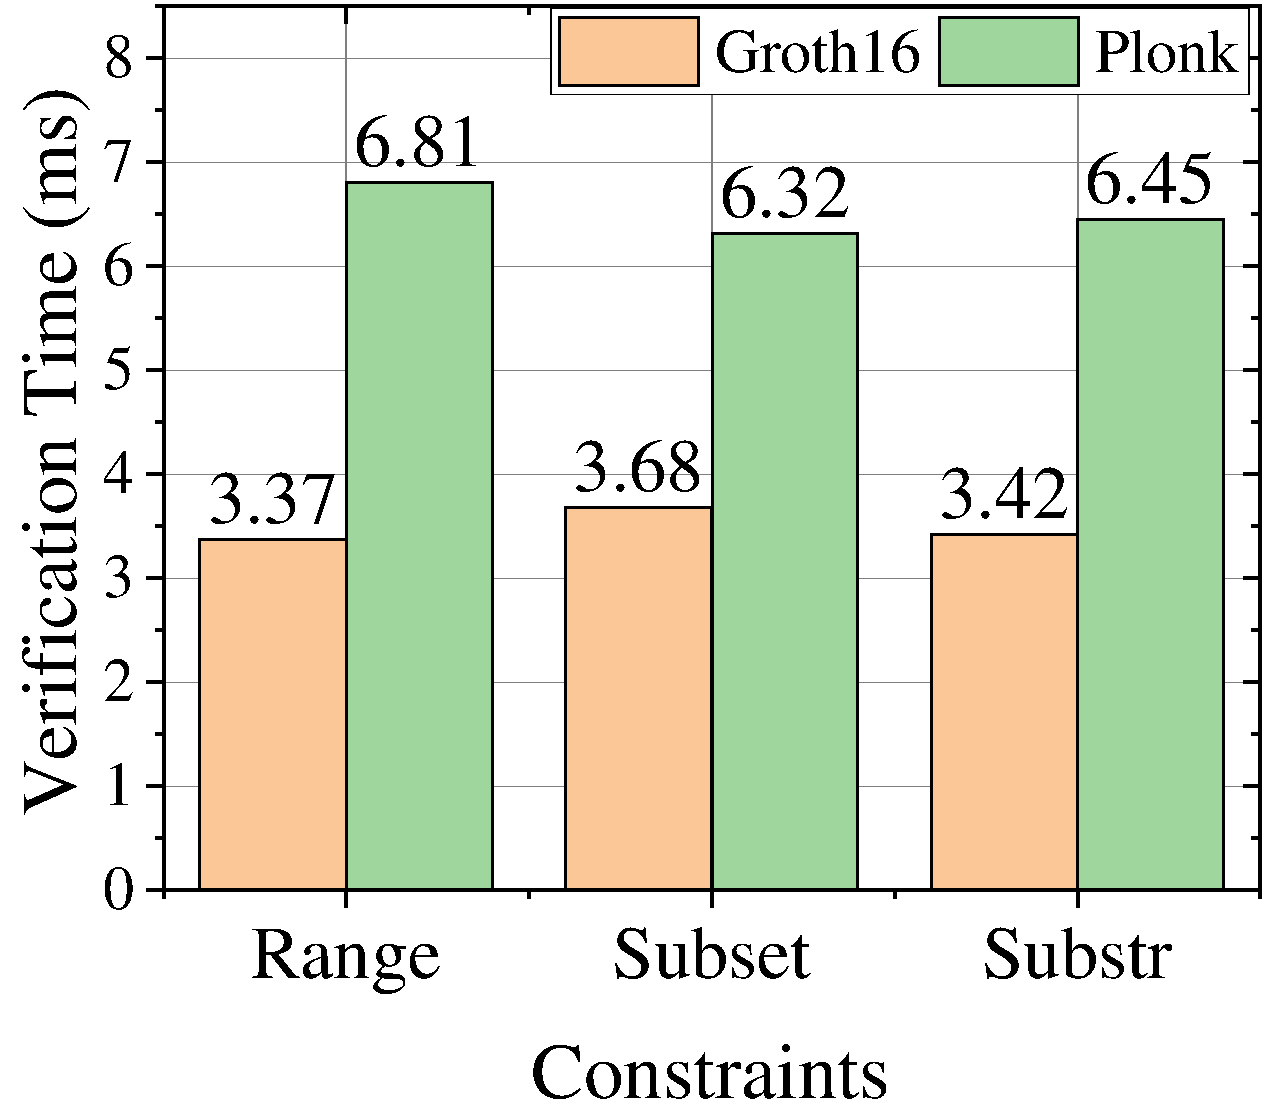
\includegraphics[width=0.4\linewidth]{figures/exp/constraint_hash_verify_time.pdf}
  }
    \subfigure[Gas Cost]{
        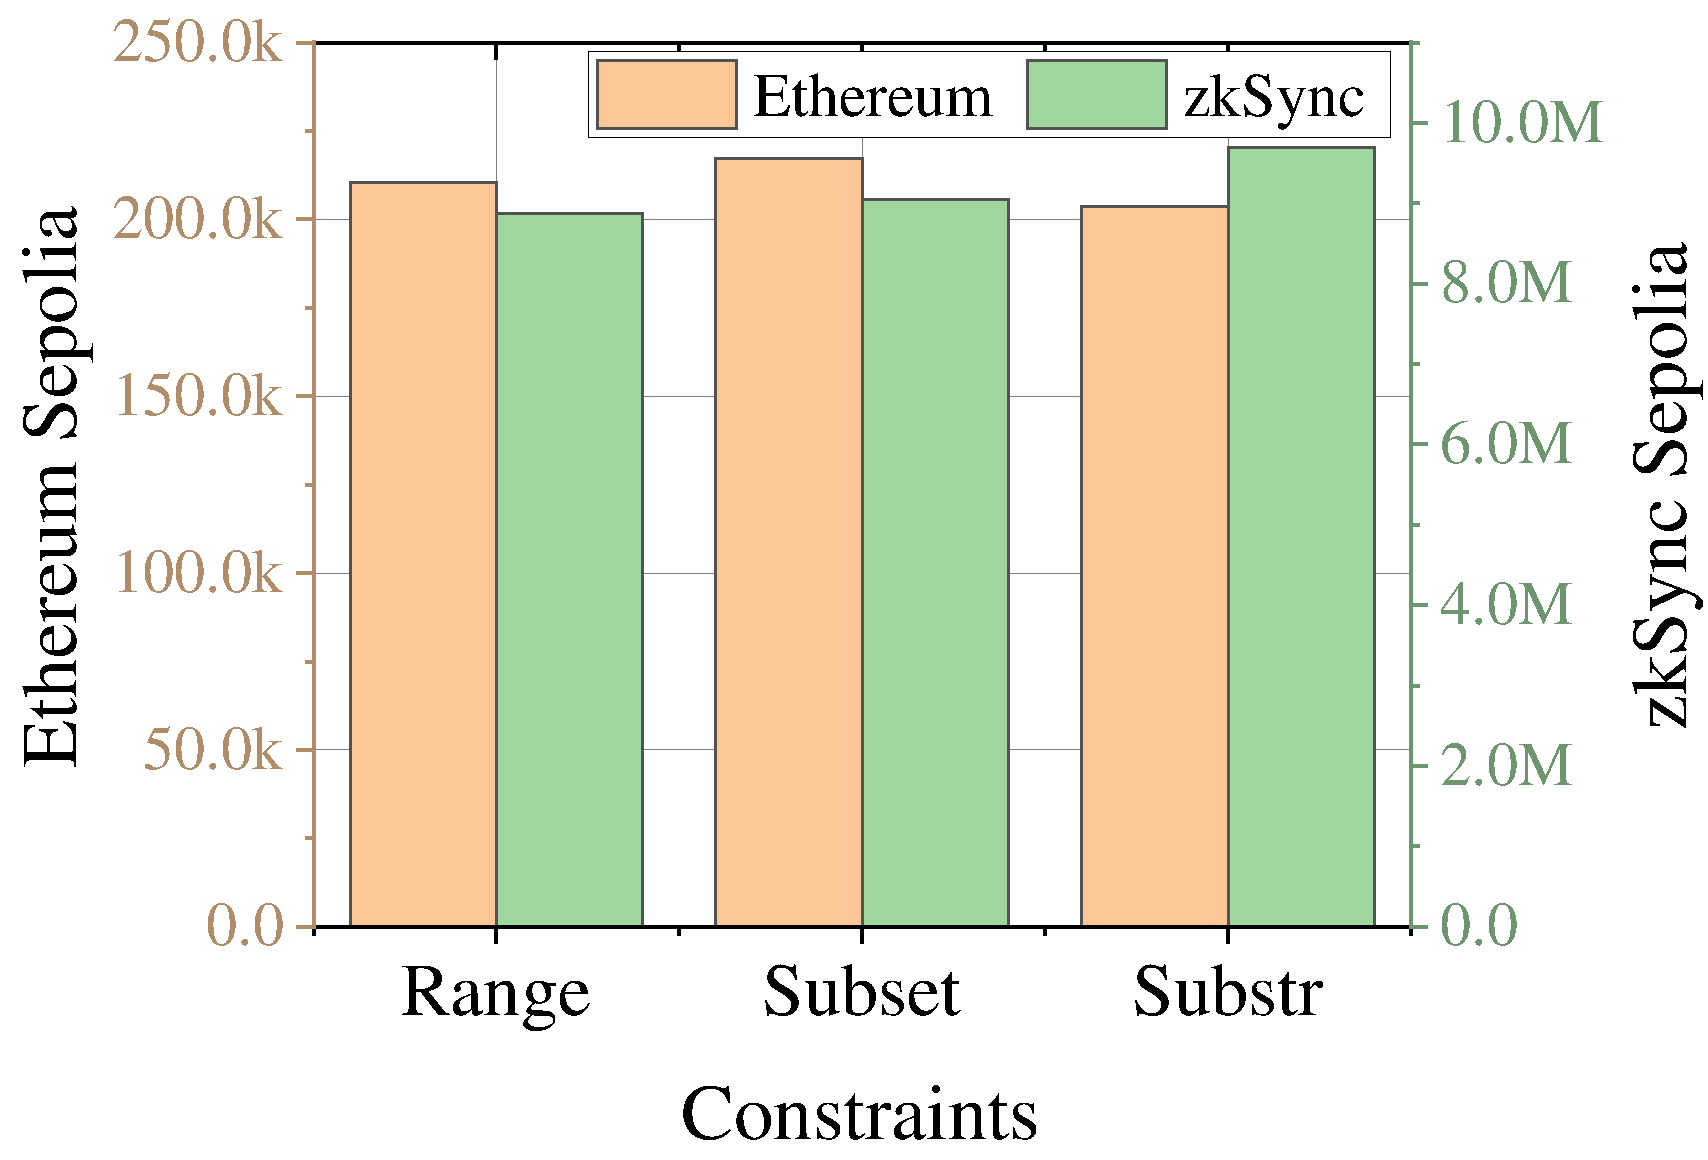
\includegraphics[width=0.52\linewidth]{figures/exp/constraint_hash_verify_gas_cost.pdf}
        \label{fig_constraint_hash_gas}
    }
    \caption{Performance of Constraint-hash Proof Verification}
    \label{fig_constraint_hash}
\end{figure}
Fig.~\ref{fig_constraint_hash_verify} demonstrates the verification time comparison between Groth16 and Plonk protocols for different proofs. The data indicates that Groth16 protocol requires approximately 3 milliseconds for proof verification, while Plonk protocol takes about 6 milliseconds. Fig.~\ref{fig_constraint_hash_gas} compares the gas consumption when verifying proofs using Solidity smart contracts on both Ethereum Sepolia and zkSync Sepolia networks. The results show that proof verification requires approximately 20,000 gas on the Ethereum network and about 1,000,000 gas on the zkSync network. Despite the difference in gas prices between these networks, the actual costs remain relatively low: approximately 0.0000274 ETH on Ethereum and 0.000904 ETH on zkSync.

\subsubsection{Root Obfuscation Proof}
To validate the efficiency of our root obfuscation proof, we conduct experiments on proof generation for our $\mathsf{IMT}$ with depths ranging from 10 to 20. The proof verification time and on-chain gas cost are similar to that discussed in the constraint-hash proof section.  The verification times  of Groth16 and Plonk protocols are approximately 3 milliseconds and 6 milliseconds respectively. Regarding the gas consumption required for verifying proofs of different depths, due to the unchanged length of public input and the succinctness property of zk-SNARKs, the verification cost is comparable to that of constraint-hash proof verification.

\begin{figure}[htbp]
    \centering
    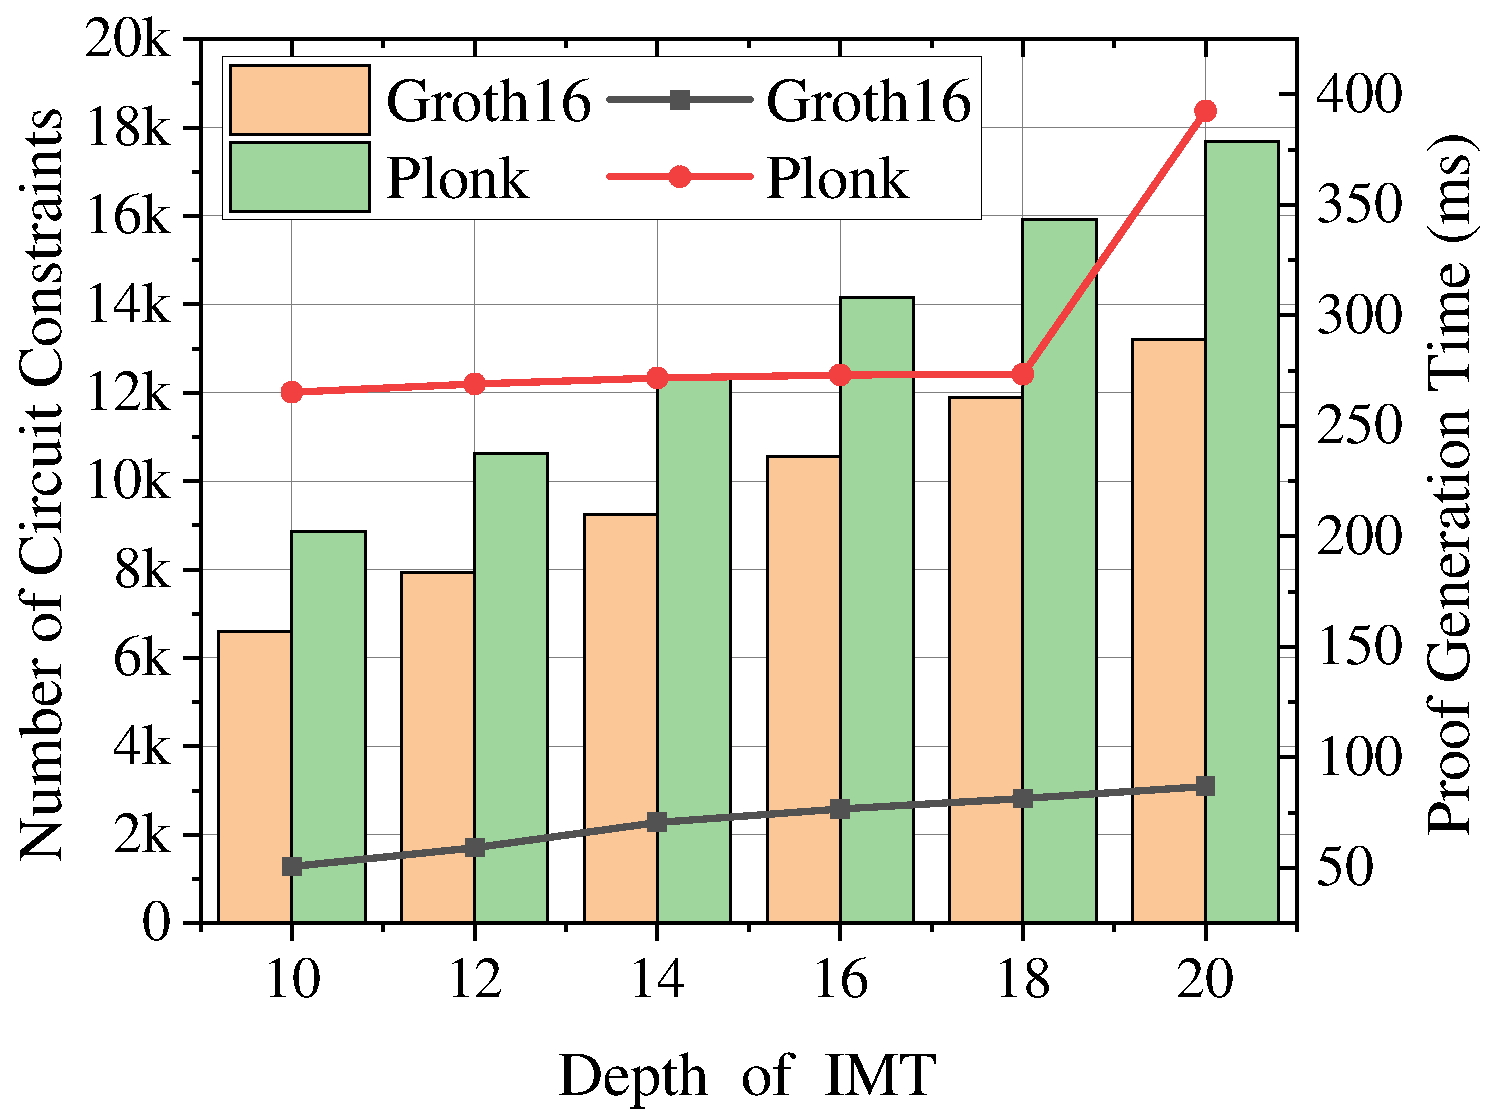
\includegraphics[width=0.8\linewidth]{figures/exp/root_obfuscation_prove_constraints.pdf}
    \caption{Proof Generation Time and Number of \emph{Circuit} Constraints with Different Depth of  $\mathsf{IMT}$}
    \label{fig_root_obfuscation_prove}
\end{figure}

Fig.~\ref{fig_root_obfuscation_prove} illustrates the performance metrics for generating root obfuscation proofs across Integrity Merkle Tree ($\mathsf{IMT}$) depths ranging from 10 to 20. The bar chart represents the number of \emph{circuit} constraints, while the line graph shows the proof generation time. Under the Groth16 protocol, as the depth increases, the number of \emph{circuit} constraints grows from 1,000 to 11,000, with corresponding proof generation time rising from 50ms to nearly 100ms. For the Plonk protocol, the \emph{circuit} constraint count increases from 9,000 to 17,000. While the proof generation time remains stable at approximately 270ms for tree depths between 10 and 18, it significantly increases to around 400ms at depth 20 due to the activation of server memory paging mechanisms. 

\subsection{On-chain Costs}
We analyze the resource consumption of key processes in our proposed solution, including contract deployment, fund locking, fund claiming, and various dispute resolution scenarios during data delivery. We conducted tests on both Ethereum Sepolia test network and zkSync Sepolia test network to simulate the actual consumption on Ethereum mainnet and zkSync mainnet respectively. According to the data presented in Table~\ref{tab_gas_cost}, our contract design demonstrates cost-efficiency on both Ethereum and zkSync networks. Notably, although gas consumption on zkSync is relatively higher, the lower gas price results in reduced ETH expenditure overall.

For various dispute resolution scenarios, the transaction overhead is critically important, as if this overhead exceeds the transaction funds in one round of the data delivery process, the punishment mechanism designed in our solution would fail to effectively constrain malicious behaviors from $\mathcal{DO}$ and $\mathcal{DR}$. Our experimental results demonstrate that as long as the funds per round exceed a specific threshold, our transaction overhead remains a small percentage of the transaction funds. In this context, when malicious behavior occurs, the affected party can penalize such behavior or claim their deserved compensation by invoking the contract at minimal cost, which substantiates the fairness and practicality of our proposed solution.


\section{Conclusion}\label{section:conclusion}
In this paper, we proposed a customizable and verifiable data trading scheme. The scheme realizes a fair and verifiable data trading process between data owners and data requesters through the use of blockchain, zk-SNARKs, smart contracts, and off-chain channels. The core of our approach is a zk-SNARK-based scheme for customized data constraints and integrity verification. By constructing a four-layer Merkle tree, we enable data owners to efficiently generate proofs, and requesters to efficiently verify that the masked data complies with their custom requirements and is derived from the endorsed raw data, all without exposing sensitive information. In addition, we designed a fair exchange mechanism through a multi-round off-chain delivery protocol. This allows data requesters to verify the quality of  data subsets during each trading round. The integrated on-chain dispute resolution mechanism, powered by zk-SNARK verification, deters malicious behavior by penalizing invalid data or withheld payments. Crucially, this design confines the financial risk of paying for low-quality data to a single subset. Through comprehensive security analysis and performance experiments, we have demonstrated that our scheme is not only efficient in zk-SNARK proof generation and on-chain operation,  but also successfully provides the desired properties of privacy preservation, verifiability, and fairness. While our framework mitigates key exchange risks, it does not fully eliminate the possibility of acquiring low-quality data. Future work will address this financial exposure by developing mechanisms that ensure payment only for verified high-quality data, thereby enhancing fairness in data trading.

\section*{Acknowledgment}
This work is supported in part by Anhui Province Key Technologies Research \& Development Program under Grant No. 2022a05020050, the National Natural Science Foundation of China under Grants No. 62372425 and No. 62501562, and Youth Innovation Promotion Association of the Chinese Academy of Sciences under Grant No. Y202093.

\bibliographystyle{IEEEtran}
\bibliography{main}

\end{document}